\documentclass[10pt,a4paper]{article}
\usepackage[utf8]{inputenc}
\usepackage[T1]{fontenc}
\usepackage[ngerman]{babel}
\usepackage{lmodern}
\usepackage{microtype}
\usepackage[a4paper,top=15mm,bottom=16mm,left=16mm,right=16mm,headheight=13pt,headsep=5mm,footskip=8mm]{geometry}
\usepackage{amsmath,amssymb,amsfonts}
\usepackage{booktabs}
\usepackage{array}
\usepackage{graphicx}
\usepackage{xcolor}
\usepackage{fancyhdr}
\usepackage{hyperref}

\definecolor{navy}{HTML}{12284C}
\definecolor{slate}{HTML}{334E68}
\definecolor{accent}{HTML}{1B5E20}
\definecolor{boxbg}{HTML}{F4F7FA}

\hypersetup{
  colorlinks=true,
  linkcolor=navy,
  urlcolor=navy,
  citecolor=navy,
  pdftitle={Das Zeitanziehungsgesetz (Time Attraction Law): Forschungsmonographie (Versionen 1 bis 21)},
  pdfauthor={David Szabolcsi}
}

\pagestyle{fancy}
\fancyhf{}
\fancyhead[L]{\footnotesize\scshape\color{slate}Das Zeitanziehungsgesetz (Time Attraction Law) --- Forschungsmonographie (V1--V21)}
\fancyhead[R]{\footnotesize\color{slate}D\'avid Szabolcsi (ORCID: 0009-0005-6300-074X)}
\fancyfoot[L]{\footnotesize\color{slate}CC BY-NC 4.0 --- Wissenschaftliches Arbeitsdokument (Okt.\ 2026)}
\fancyfoot[R]{\footnotesize\bfseries\color{navy}Seite \thepage\ von 15}
\renewcommand{\headrulewidth}{0.4pt}
\renewcommand{\footrulewidth}{0.4pt}

\setlength{\parindent}{0pt}
\setlength{\parskip}{2.8pt}

\newcommand{\chaphead}[2]{%
  \noindent{\color{navy}\rule{\linewidth}{1.1pt}}\par\vspace{1.5pt}%
  \noindent{\Large\bfseries\color{navy}#1}\par\vspace{1pt}%
  \noindent{\footnotesize\itshape\color{slate}#2}\par\vspace{1.5pt}%
  \noindent{\color{navy}\rule{\linewidth}{0.4pt}}\par\vspace{3pt}%
}

\begin{document}

% ==================== PAGE 1: TITLE PAGE ====================
\thispagestyle{empty}
\vspace*{-2mm}
\noindent{\color{navy}\rule{\linewidth}{2pt}}\par\vspace{1.5mm}
\begin{center}
  {\footnotesize\scshape\color{slate}Wissenschaftliche Forschungsmonographie $\cdot$ Beobachtungs-, Kompaktobjekt- \& Laborprogramm}\par\vspace{1.5mm}
  {\Large\bfseries\color{navy}DAS ZEITANZIEHUNGSGESETZ (TIME ATTRACTION LAW)}\par\vspace{1.2mm}
  {\large\bfseries\color{slate}Dichtemodulierte Zeitstr\"omung, die $C$-Kopplungskonstante ($C$ coupling constant),}\\
  {\large\bfseries\color{slate}positiv-definite 3D-Top-Hat-Gl\"attung, galaktische Rotationskurven, Multi-Quellen-Gammastrahlen-Timing,}\\
  {\large\bfseries\color{slate}Neutronenstern-Gleichgewicht sowie Granitkammer-Atomuhren- und Acht-Spulen-Magnetfeld-Experimente}\par\vspace{2mm}
  {\normalsize\bfseries D\'avid Szabolcsi}\par\vspace{1mm}
  {\small Unabh\"angiger Forscher, Unterterzen, Schweiz}\par
  {\small ORCID: \href{https://orcid.org/0009-0005-6300-074X}{\texttt{0009-0005-6300-074X}} $\cdot$ GitHub: \href{https://github.com/unbekanntedavid-glitch/Time-Attraction}{\texttt{unbekanntedavid-glitch/Time-Attraction}}}\par
  {\small 24.\ Oktober 2026}
\end{center}
\vspace{1.5mm}
\noindent{\color{navy}\rule{\linewidth}{0.8pt}}\par\vspace{1mm}

{\small\noindent{\bfseries\color{navy}\"Uberblick}\par
Ich stelle das \textbf{Zeitanziehungsgesetz (Time Attraction Law)} als offenes Forschungsprogramm vor, das auf einer pr\"azisen Dichtegl\"attungsvorschrift beruht und das ich in einundzwanzig aufeinander aufbauenden Forschungsschritten (Versionen 1 bis 21) entwickelt habe. Die Berechnungen in dieser kompakten Forschungsmonographie pr\"ufen ausgew\"ahlte Gleichgewichts- und Beobachtungskopplungen; sie begr\"unden noch keine geschlossene kovariante Theorie und keinen experimentellen Nachweis eines zus\"atzlichen Uhreneffekts. Im gesamten Text unterscheide ich algebraische Resultate von Modellannahmen sowie numerische Pr\"ufungen von experimentellen Belegen: Die archivierten Rechnungen dokumentieren, was getestet wurde, w\"ahrend die offenen Aufgaben benennen, was noch erforderlich ist, um diese Ergebnisse in einer gemeinsamen Dynamik zu verbinden. Meine physikalische Grundannahme lautet, dass die Zeit das prim\"are physikalische Medium ist, dessen lokale Str\"omungsdichte durch die umgebende Masse-Energie-Verteilung angezogen und verlangsamt wird. Hier fasse ich die physikalische Motivation (einschlie\ss lich der separaten spekulativen Biokoh\"arenz-Hypothese aus V13--V16), die Cauchy-Exponentialform und die \textbf{$C$-Kopplungskonstante}, das positiv-definite 3D-Kugel-Top-Hat-Gesetz, bedingte Skalenabsch\"atzungen \"uber SPARC-Galaxien, das Sonnensystem, Neutronensterne und die $300\,\text{mm}$-Acht-Spulen- und Granitkammer-Laboranordnung, die offenen Aufgaben (a)--(d) sowie das im Anhang beigef\"ugte KI-gest\"utzte technische Reproduktions-Audit zusammen.

\vspace{0.5mm}
\noindent{\bfseries\color{navy}Prim\"are reproduzierbare Archiv-Datens\"atze (Zenodo-DOIs \& Versionslinie)}
\begin{center}\vspace{-2pt}
{\footnotesize
\begin{tabular}{@{}>{\bfseries}p{0.15\linewidth}p{0.27\linewidth}p{0.53\linewidth}@{}}
\toprule
Stufe & Zenodo-DOI / Kennung & Wissenschaftlicher Umfang \& Gepr\"ufte Inhalte \\
\midrule
V1--V13 & GitHub-Serienarchiv & Exponentieller Cauchy-Ansatz, Schwachfeld-/Horndeski-Abbildungen, fr\"uhe Uhrentests. \\
V14--V16 & \texttt{10.5281/zenodo.23217189} & Dichtebedingte Zeitkoh\"arenz, $C$-Kopplungskonstanten-Faktor, Biokoh\"arenz-Schicht $\Phi_t$. \\
V17 & \texttt{10.5281/zenodo.19666220} & 155 SPARC-Galaxien-Rotationskurven (123 blind) \& Multi-Quellen-H.E.S.S.-Timing-Audit. \\
V19 (7.\ Modell) & \texttt{10.5281/zenodo.23497128} & Positiv-definites 3D-Top-Hat-Gesetz $f_L=\exp(-\gamma_L\bar{\rho}_L)$ f\"ur alle 175 SPARC-Galaxien. \\
V20 (GH V18) & \texttt{10.5281/zenodo.23540741} & 8-Spulen-Magnetfeldenergetik ($\Delta y=-1{,}2017\times 10^{-48}$) \& Granit-Atomuhrenkammer. \\
V21 (GH V19/21) & \texttt{10.5281/zenodo.23602501} & 33 Neutronenstern-TOV-Sequenzen, Chandrasekhar-Stabilit\"at, Sirius B / NICER \& offene Punkte. \\
\bottomrule
\end{tabular}}
\end{center}

\vspace{1mm}
\noindent{\bfseries\color{navy}Drei zentrale physikalische Fragen dieser Monographie}
\begin{itemize}\setlength{\itemsep}{1.5pt}\setlength{\parskip}{0pt}\setlength{\topsep}{1pt}
  \item \textbf{1. Warum verschiebt sich die Uhrenfrequenz? (Das physikalische ,,Warum``):} In Kapitel 2 untersuche ich, ob das Zeitanziehungsgesetz ein Skalarfeld, ein effektives Zeitfluid oder ein brechendes Raumzeit-Medium beschreibt, und wie das algebraisch fixierte ,,Wie`` ($f_L = \exp(-\gamma_L \bar{\rho}_L)$) mit der offenen kovarianten Wirkungsschlie\ss ung (Aufgabe \texttt{50aa2db0}) zusammenh\"angt.
  \item \textbf{2. Wie passt das Modell \"uber verschiedene Gr\"o\ss enskalen zusammen?:} In den Kapiteln 4, 5 und 10 zeige ich, wie der 3D-Kugel-Top-Hat-Kern galaktische Kiloparsec-Skalen, bedingte Skalenabsch\"atzungen im Sonnensystem und Labormessungen am $300\,\text{mm}$-Spulenflansch sowie an der Granitkammer verbindet.
  \item \textbf{3. Welche spezifischen Vorhersagen unterscheiden es von $\Lambda$CDM?:} In den Kapiteln 6--10 quantifiziere ich Vorhersagen f\"ur VHE-Gammaphotonen-Laufzeiten, Masse-Radius- und Pulsationsverschiebungen kompakter Sterne sowie polarit\"atsgerade Labor-Frequenzverschiebungen.
\end{itemize}
}\vfill
\noindent{\color{navy}\rule{\linewidth}{0.6pt}}\par
\noindent{\scriptsize\color{slate}\textbf{Lizenz- \& Rechtshinweis:} Dieses Werk ist lizenziert unter Creative Commons Namensnennung -- Nicht-kommerziell 4.0 International (\textbf{CC BY-NC 4.0}). S\"amtliche kommerziellen, industriellen und technologischen Verwertungsrechte verbleiben ausdr\"ucklich beim Autor, D\'avid Szabolcsi.}
\newpage

% ==================== PAGE 2: TABLE OF CONTENTS & NOTATION ====================
\chaphead{Inhaltsverzeichnis \& Bezeichnungen}{Aufbau der Monographie, fundamentale Gr\"o\ss en und methodischer Rahmen}

\noindent{\bfseries\color{navy}Inhalt dieser Monographie}\par\vspace{1pt}
{\footnotesize
\begin{tabular}{@{}>{\bfseries\color{navy}}p{0.12\linewidth}p{0.76\linewidth}>{\raggedleft\arraybackslash\bfseries}p{0.08\linewidth}@{}}
\toprule
Abschnitt & Kapiteltitel & Seite \\
\midrule
Titelseite & Titelseite, \"Uberblick \& Reproduzierbare Archiv-Linie & 1 \\
Inhalt & Inhaltsverzeichnis, Bezeichnungen \& Methodische Grunds\"atze & 2 \\
Kapitel 1 & Versionsgeschichte von V1 bis V21: Die Entwicklung meines Forschungsprogramms & 3 \\
Kapitel 2 & Kern der Theorie: Das physikalische ,,Warum`` \& die Bewusstseinskoh\"arenz & 4 \\
Kapitel 3 & Exponentialform, Definition der $C$-Kopplungskonstanten und Normierung & 5 \\
Kapitel 4 & L\"osung des Problems negativer Dichten \& Skalen\"ubergreifende Einordnung & 6 \\
Kapitel 5 & Galaktische Rotationskurven: Auswertung von 155 SPARC-Galaxien \& 3D-Top-Hat-Gitter & 7 \\
Kapitel 6 & Hochenergetisches Gammastrahlen-Timing: Multi-Quellen-H.E.S.S.-Datenanalyse & 8 \\
Kapitel 7 & Neutronenstern-Modellierung in V21: TOV-Sequenzen \& Datensatz-Inventar & 9 \\
Kapitel 8 & St\"orungsrechnung: Anisotrope Spannung \& Radiale Chandrasekhar-Stabilit\"at & 10 \\
Kapitel 9 & Bedingte Uhren- \& Rotverschiebungs-Hypothesen: Sirius B und NICER-Likelihoods & 11 \\
Kapitel 10 & Geplante Labormessungen: Acht-Spulen-Magnetfeld \& Granit-Atomuhrenkammer & 12 \\
Kapitel 11 & Offene theoretische und experimentelle Fragen: Aufgaben (a)--(d) & 13 \\
Kapitel 12 & Ausblick: Der unmittelbare n\"achste physikalische Schritt (\texttt{50aa2db0}) & 13 \\
Anhang & KI-gest\"utztes technisches Reproduktions-Audit (Deutsche \"Ubersetzung, Runde 3) & 14--15 \\
\bottomrule
\end{tabular}}

\vspace{1.5mm}
\noindent{\bfseries\color{navy}Grundbegriffe und mathematische Symbole}\par
Zur klaren Unterscheidung aller Gr\"o\ss en verwende ich in dieser Monographie durchg\"angig die folgende Notation:
\begin{center}\vspace{-2pt}
{\footnotesize
\begin{tabular}{@{}>{\bfseries}p{0.28\linewidth}p{0.24\linewidth}p{0.43\linewidth}@{}}
\toprule
Begriff & Symbol / Definition & Physikalische Rolle im Zeitanziehungsgesetz \\
\midrule
Zeitanziehungsgesetz & $f_L(\mathbf{x}) = \exp(-\gamma_L \bar{\rho}_L(\mathbf{x}))$ & Gesetz, das die lokale Zeitstr\"omungsdichte mit der gegl\"atteten Dichte verkn\"upft. \\
$C$-Kopplungskonstante & $C \equiv \frac{4\pi G}{c^2} = 9{,}331988\times 10^{-27}\,\text{m/kg}$ & Definierte Kopplungskonstante ($G/c^2 = 7{,}426160\times 10^{-28}\,\text{m/kg}$; verschieden von $C_{\text{amp}}(\rho)$). \\
Skalenkopplung ($\alpha=1$) & $\gamma_L = \alpha\frac{G L^2}{c^2} = \frac{C L^2}{4\pi}\;(\alpha=1)$ & Skalenabh\"angiger D\"ampfungskoeffizient ($\text{m}^3\,\text{kg}^{-1}$) f\"ur Gl\"attungsradius $L$ ($\neq \mathcal{L}_{\text{like}}$). \\
3D-Top-Hat-Dichte & $\bar{\rho}_L(\mathbf{x}) = \frac{3}{4\pi L^3}\int_{|\mathbf{y}-\mathbf{x}|\le L}\rho(\mathbf{y})\,d^3y$ & Nicht-negatives Kugelschnittmittel der Massendichte $\rho$ (bzw.\ Energiedichte $\varepsilon/c^2$). \\
Bewusstseinskoh\"arenz & $\Phi_t,\,\Phi_B,\,\kappa$ & Fr\"uhe spekulative Biokoh\"arenz-Potenzialgr\"o\ss e, Magnetfluss und Raumkr\"ummung. \\
\bottomrule
\end{tabular}}
\end{center}

\vspace{2mm}
\noindent{\bfseries\color{navy}Methodische Grunds\"atze: Reproduzierbarkeit und offene Fragen}\par
Bei der Darstellung dieses Rahmens trenne ich strikt zwischen dem, was bereits in hash-gepr\"uftem, reproduzierbarem Code fixiert ist, und dem, was eine offene theoretische oder experimentelle Aufgabe bleibt:
\begin{enumerate}\setlength{\itemsep}{2pt}\setlength{\parskip}{0pt}\setlength{\topsep}{2pt}
  \item \textbf{Das gepr\"ufte ,,Wie`` ist reproduzierbar fixiert:} In meinen Zenodo-Archiven und meinem GitHub-Repository stelle ich deterministische Skripte, SHA-256-Manifeste und numerische Quadraturpr\"ufungen bereit, die festlegen, \emph{wie} das Zeitanziehungsgesetz die Massendichte $\rho(\mathbf{x})$ auf den beschr\"ankten Faktor $0 < f_L(\mathbf{x}) \le 1$ abbildet.
  \item \textbf{Jede Version ist ein Zwischenschritt:} Keine Ausgabe meiner V1--V21-Reihe wird als geschlossen betrachtet. Jede Version pr\"uft eine mathematische Hypothese gegen Beobachtungs- oder Laborschranken, dokumentiert ihre Grenzen offen und verfeinert die Formulierung entsprechend.
  \item \textbf{KI-gest\"utzte technische Reproduktions-Audits:} Technische Reproduktions- und Manuskriptpr\"ufungen mit Unterst\"utzung von Academia Co-scientist (keine institutionelle Zeitschriften-Begutachtung) dienten als diagnostische Werkzeuge. Als diese Pr\"ufungen den Unterschied zwischen 1D-Mittelebenen-Proxy und 3D-Top-Hat in V19, den magnetischen Kreuzterm $2\mathbf{B}_{\text{bg}}\cdot\mathbf{B}_{\text{coil}}$ in V20 oder die n\"aherungsweisen Pulsationsoperatoren und die offene kovariante Wirkungsschlie\ss ung in V21 aufzeigten, habe ich diese Korrekturen direkt in Code und Dokumentation \"ubernommen. Die deutsche \"Ubersetzung des technischen Audits der 3.\ Runde ist auf den Seiten 14 und 15 abgedruckt.
\end{enumerate}
\newpage

% ==================== PAGE 3: CHAPTER 1 (VERSION HISTORY V1-V21) ====================
\chaphead{Kapitel 1: Versionsgeschichte von V1 bis V21}{Der iterative Entwicklungsweg des Zeitanziehungsgesetzes \"uber einundzwanzig Forschungsstufen}

Damit der Leser den genauen Verlauf meiner Forschung nachvollziehen kann, fasse ich hier zusammen, wie sich das \textbf{Zeitanziehungsgesetz (Time Attraction Law)} vom ersten mathematischen Ansatz in Version 1 bis zu den Kompaktobjekt- und Laborpaketen in Version 21 entwickelt hat. Jede Stufe diente als Pr\"ufstein, der zeigte, was tragf\"ahig war und was korrigiert werden musste.

\begin{center}\vspace{-2pt}
{\footnotesize
\begin{tabular}{@{}>{\bfseries\color{navy}}p{0.14\linewidth}p{0.25\linewidth}p{0.56\linewidth}@{}}
\toprule
Versionsstufe & Prim\"arer Fokus & Erreichte Meilensteine, Erkenntnisse \& Selbstkorrekturen \\
\midrule
V1 -- V4 & Multiplikativer Cauchy-Ansatz & Ich formulierte das Postulat, dass unabh\"angige lokale Massendichten multiplikativ auf den Zeitfluss wirken, $f(\rho_1+\rho_2)=f(\rho_1)f(\rho_2)$, woraus $f(\rho)=\exp(-\gamma\rho)$ folgt. \\
V5 -- V7 & Schwachfeld- \& Cham\"aleon-Studien & Untersuchung von Skalar-Tensor- und Abschirmungs-Analogien, um lokale Dichtegradienten mit effektiven Beschleunigungen in d\"unnen Umgebungen zu verbinden. \\
V8 -- V12 & Horndeski- \& Zeitdilatations-Modelle & Untersuchung effektiver Lapse-Modifikationen und Horndeski-inspirierter Kopplungen anhand optischer Uhrenvergleiche. \\
V13 -- V16 & Dichtebedingte Zeitkoh\"arenz \& Biokoh\"arenz ($\Phi_t$) & (\texttt{10.5281/zenodo.23217189}) Einf\"uhrung der \textbf{$C$-Kopplungskonstanten} ($C=4\pi G/c^2$), des Verst\"arkers $C_{\text{amp}}(\rho)=1+C_0 e^{-\rho/\rho_c}$ ($C_0=5$) und der Biokoh\"arenz-Hypothese ($\Phi_t$, $\Phi_B$, $\kappa$, EEG/HRV). Sp\"atere Pr\"ufungen zeigten, dass lineare Differentialformen $\rho<0$-Vorzeichenwechsel erzeugen und $C_0=5$ flache Rotationskurven \"ubersch\"atzt. \\
V17 & SPARC-155-Galaxien- \& H.E.S.S.-Audit & (\texttt{10.5281/zenodo.19666220}) Auswertung von 175 SPARC-Galaxien (155 qualit\"atsgefilterte Kurven; 123 blinde Testgalaxien mit 2596 Punkten) und f\"unf H.E.S.S./MAGIC-Gammaquellen (PKS 2155-304, Mrk 501, Vela, Crab, GRB 190114C). \\
V18 (Intern) & Gl\"attungskern-Neuformulierung & Test integraler Gl\"attungskerne zur Vermeidung numerischen Ableitungsrauschens und unphysikalischer negativer Effektivdichten an scharfen R\"andern. \\
V19 (7.\ Modell) & Positiv-definites 3D-Kugel-Top-Hat-Gesetz & (\texttt{10.5281/zenodo.23497128}) L\"osung des Problems negativer Dichten durch Definition von $\bar{\rho}_L(\mathbf{x})$ als 3D-Kugel-Top-Hat-Integral \"uber Radius $L$, was $\bar{\rho}_L\ge 0$ und $0<f_L\le 1$ garantiert; Auswertung auf allen 175 SPARC-Galaxien. \\
V20 (GH V18) & 8-Spulen-Magnetfeld \& Granit-Uhrenkammer & (\texttt{10.5281/zenodo.23540741}) Entwurf des Laborprogramms: bewegliche Granitkammer um eine Atomuhr und 8-Spulen-Magnetfeldenergetik-Test ($\varnothing 300\,\text{mm}$ Flansch, $\Delta y = -1{,}2017108\times 10^{-48}$ bei $L=0{,}631\,\text{m}$), gepr\"uft in drei technischen Audit-Runden. \\
V21 (GH V19/21) & Neutronenstern-TOV, St\"orungen \& Offene Punkte & (\texttt{10.5281/zenodo.23602501}) Erweiterung des 3D-Top-Hat-Gesetzes auf 33 Neutronenstern-TOV-Sequenzen (SLy, APR4, H4), $X$-Sektor-Spannungsrekonstruktion, radiale Pulsationen ($\omega_0^2$), Sirius B / NICER und vier offene Aufgaben (a)--(d). \\
\bottomrule
\end{tabular}}
\end{center}

\noindent{\bfseries\color{navy}Drei methodische Wendepunkte meiner Forschungsarbeit}\par
Im R\"uckblick auf V1--V21 pr\"agen drei methodische Wendepunkte die Weiterentwicklung des Programms:
\begin{enumerate}\setlength{\itemsep}{1.5pt}\setlength{\parskip}{0pt}\setlength{\topsep}{1pt}
  \item \textbf{Von differentiellen Proxys zur positiv-definiten Integralgl\"attung (V13 $\to$ V19):} In fr\"uhen Versionen f\"uhrten Laplace-Ableitungen oder lokale Mittelebenen-Proxys zu Vorzeichenwechseln mit negativer Effektivdichte. Durch das 3D-Kugel-Top-Hat-Mittel $\bar{\rho}_L$ in V19 ist $0 < f_L(\mathbf{x}) \le 1$ in jedem Raumpunkt mathematisch gesichert.
  \item \textbf{Von Einzelanpassungen zu blinden Multi-Objekt-Kontrollen (V16 $\to$ V17/V19):} Statt Parameter an einzelne Galaxien oder einen einzelnen Blazar-Flare anzupassen, habe ich die Masse-Leuchtkraft-Verh\"altnisse ($\Upsilon_{\text{disk}}=0{,}5$, $\Upsilon_{\text{bulge}}=0{,}7\,M_\odot/L_\odot$) fixiert und PKS 2155-304 mit vier weiteren Gammaquellen abgeglichen.
  \item \textbf{Von algebraischen Rezepten zu expliziten offenen Randbedingungen (V20 $\to$ V21):} In V20 und V21 habe ich jede Rechnung mit SHA-256-Pr\"ufsummen versehen und die fixierten algebraischen Profile klar von der offenen kovarianten Wirkungsableitung (Aufgabe \texttt{50aa2db0}) getrennt.
\end{enumerate}
\newpage

% ==================== PAGE 4: CHAPTER 2 (CORE ESSENCE, PHYSICAL WHY & CONSCIOUSNESS COHERENCE) ====================
\chaphead{Kapitel 2: Kern der Theorie --- Das ,,Warum`` \& Biokoh\"arenz}{Warum Masse-Energie-Dichte den Zeitfluss moduliert, die Medium-Interpretation und die spekulative Biokoh\"arenz-Schicht}

Eine physikalische Untersuchung muss neben der formalen Rechenvorschrift auch die physikalische Motivation benennen. Im \textbf{Zeitanziehungsgesetz (Time Attraction Law)} gehe ich von einer ontologischen Pr\"amisse aus: \textbf{Die Zeit ist keine blo\ss{} passive mathematische Koordinate, sondern der prim\"are physikalische Tr\"ager, dessen lokale Str\"omungsdichte durch Masse-Energie-Dichte angezogen und verdichtet wird.}

\noindent{\bfseries\color{navy}1. Das physikalische ,,Warum``: Feld, Zeitfluid oder brechendes Raumzeit-Medium?}\par
In der Allgemeinen Relativit\"atstheorie (ART) kr\"ummt Masse-Energie die Raumzeit gem\"a\ss{} $G_{\mu\nu} = \frac{8\pi G}{c^4}T_{\mu\nu}$, und die gravitative Zeitdilatation folgt aus der Metrikkomponente $g_{00}$. In meinem Ansatz frage ich, welcher Mechanismus eine zus\"atzliche lokale Verlangsamung von Uhren bewirken kann, wenn sich Masse-Energie innerhalb einer Wechselwirkungsumgebung vom Radius $L$ konzentriert. Ich interpretiere den Zeitfluss als Medium mit einer effektiven lokalen Tr\"agerdichte (analog zu einem optischen Medium mit Brechungsindex $n_t(\mathbf{x}) = f_L(\mathbf{x})^{-1} = \exp(+\gamma_L \bar{\rho}_L(\mathbf{x}))$ oder einem kompressiblen Zeitfluid). Wo sich Masse-Energie-Dichte $\rho(\mathbf{x}) = T_{00}/c^2$ konzentriert, zieht sie das zeitliche Medium innerhalb der Mittelungskugel vom Radius $L$ an. Dadurch wird die lokale Eigenzeitrate relativ zu einer Vakuum-Referenzuhr ged\"ampft gem\"a\ss :
\begin{equation}
  f_L(\mathbf{x}) \;=\; \exp\!\bigl(-\gamma_L\,\bar{\rho}_L(\mathbf{x})\bigr), \qquad \gamma_L \;=\; \frac{G L^2}{c^2} \;=\; \frac{C\,L^2}{4\pi},
\end{equation}
wobei $C \equiv 4\pi G/c^2$ die \textbf{$C$-Kopplungskonstante} ist.

\noindent{\bfseries\color{navy}2. Trennung zwischen dem gepr\"uften ,,Wie`` und dem dynamischen ,,Warum`` (Aufgabe \texttt{50aa2db0})}\par
Wissenschaftliche Sorgfalt erfordert die Trennung zwischen algebraisch fixierten Rezepten und einer feldtheoretischen Ableitung. In V19--V21 habe ich das funktionale \textbf{,,Wie``} fixiert --- die nichtlokale Abbildung $\rho(\mathbf{x}) \to \bar{\rho}_L(\mathbf{x}) \to f_L(\mathbf{x})$. In den gepr\"uften Neutronenstern-Rezepten sichert die hydrostatische Gleichung $P' = -(\varepsilon+P)\nu'$ zwar bereits die separate Erhaltung des Materietensors ($\nabla_\mu T^{\mu\nu}_{\text{matter}} = 0$). Wenn jedoch die Metrikfunktionen ($\nu'$ oder $m'$) ohne Skalar-Tensor-Wirkung durch $f_L(r)$ modifiziert werden, bleibt die rechte Seite der Einstein-Gleichungen ohne einen effektiven Zusatzsektor $T^{\mu\nu}_X$ ($\nabla_\mu(T^{\mu\nu}_{\text{matter}} + T^{\mu\nu}_X) = 0$) ungeschlossen. Das dynamische \textbf{,,Warum``} ist daher als offene Aufgabe \texttt{50aa2db0} formuliert: die Ableitung der Hintergrundgleichungen, des $X$-Sektors und der Materiekopplungen aus einem gemeinsamen kovarianten Wirkungsprinzip.

\noindent{\bfseries\color{navy}3. Spekulative Hypothesenschicht: Die Bewusstseinskoh\"arenz-Br\"ucke ($\Phi_t$, $\Phi_B$, $\kappa$)}\par
In den Versionen 13 bis 16 (und dokumentiert in der Linie von V17) habe ich dar\"uber hinaus eine spekulative konzeptionelle Frage betrachtet: Wenn die lokale Zeitstr\"omungsdichte ein physikalisches Medium ist, k\"onnen dann auch koh\"arente elektromagnetische und biologische Informationsstrukturen an diesen Tr\"ager koppeln? In dieser Hypothesenschicht f\"uhrte ich das \textbf{Bewusstseinskoh\"arenz-Potenzial} $\Phi_t$ neben dem magnetischen Fluss $\Phi_B$ und der Raumkr\"ummung $\kappa$ in eine erweiterte Quellendichte ein:
\begin{equation}
  \rho_{\text{eff}} \;=\; \rho \;+\; \Xi\,\varepsilon_0\,\Phi_t \;+\; \beta\,\Phi_B \;+\; \gamma\,\kappa, \qquad
  T_{\mu\nu}^{\text{total}} \;=\; T_{\mu\nu}^{\text{matter}} \;+\; T_{\mu\nu}^{\text{flux}} \;+\; T_{\mu\nu}^{\text{thought}},
\end{equation}
wobei $\Xi$ den Kopplungskoeffizienten und $\varepsilon_0$ die Vakuumpermittivit\"at bezeichnet. Innerhalb dieser Idee fungieren neuronale und kardiale Oszillatoren (beschrieben durch EEG-Gamma/Theta-Synchronie und Herzfrequenzvariabilit\"at, HRV) als empfindliche Phasendetektoren lokaler zeitlicher Koh\"arenz.

\noindent{\bfseries\color{navy}4. Klare methodische Abgrenzung zwischen gepr\"ufter Physik und spekulativer Perspektive}\par
In meinem Forschungsprogramm ziehe ich eine strikte Grenze zwischen beiden Ebenen:
\begin{itemize}\setlength{\itemsep}{1.5pt}\setlength{\parskip}{0pt}\setlength{\topsep}{1pt}
  \item \textbf{Quantitativer physikalischer Kern (V19--V21):} Alle numerischen Ergebnisse zu SPARC-Galaxien, H.E.S.S.-Timing, Neutronensternen sowie zum Granitkammer- und 8-Spulen-Laborexperiment beruhen \emph{ausschlie\ss lich} auf der baryonischen und elektromagnetischen Massendichte $\rho = T_{00}/c^2$ mit $\Phi_t \equiv 0$.
  \item \textbf{Spekulative Biokoh\"arenz-Schicht (V13--V16):} Die Gr\"o\ss en ($\Phi_t$, $T_{\mu\nu}^{\text{thought}}$, EEG/HRV-Biokoh\"arenz) bleiben eine ungepr\"ufte konzeptionelle Hypothese aus der fr\"uhen Entwicklungsgeschichte des Modells.
\end{itemize}
\newpage

% ==================== PAGE 5: CHAPTER 3 (DERIVATION OF THE C COUPLING CONSTANT) ====================
\chaphead{Kapitel 3: Exponentialform, Definition von $C$ und Normierung}{Herleitung der Exponentialform aus der Cauchy-Funktionalgleichung, Definition von $C$ und das Postulat $\alpha=1$}

Hier trenne ich drei mathematische Schritte klar voneinander: (1) die Herleitung der exponentiellen Funktionsform aus multiplikativen Postulaten, (2) die Definition der Konstanten $C \equiv 4\pi G/c^2$ und (3) die explizite Normierungsannahme $\alpha = 1$ in $\gamma_L = \alpha (G/c^2)L^2$, gefolgt von der Pr\"ufung des historischen Verst\"arkers $C_{\text{amp}}(\rho)$ aus V14--V16.

\noindent{\bfseries\color{navy}1. Herleitung der Exponentialform aus der Cauchy-Funktionalgleichung}\par
Ich betrachte eine Referenzuhr im Vakuum ($\rho = 0$) mit der Eigenzeitrate $d\tau_0$ und eine baugleiche Uhr innerhalb eines Bereichs, dessen gegl\"attete Masse-Energie-Dichte im Radius $L$ den Wert $\bar{\rho}_L \ge 0$ hat. Sei $f(\bar{\rho}_L) = d\tau / d\tau_0$ der dimensionslose D\"ampfungsfaktor. Ich setze drei Postulate voraus:
\begin{enumerate}\setlength{\itemsep}{1pt}\setlength{\parskip}{0pt}\setlength{\topsep}{1pt}
  \item \textbf{Vakuumnormierung:} Ohne Masse-Energie ($\bar{\rho}_L = 0$) vergeht die Zeit mit der unged\"ampften Referenzrate, also $f(0) = 1$.
  \item \textbf{Multiplikative \"Uberlagerung:} Tragen zwei unabh\"angige Massenverteilungen die gegl\"atteten Dichten $\rho_1$ und $\rho_2$ innerhalb der Wechselwirkungskugel bei, so wirkt ihre D\"ampfung multiplikativ:
  \begin{equation}
    f(\rho_1 + \rho_2) \;=\; f(\rho_1)\,f(\rho_2) \qquad \forall\,\rho_1,\rho_2 \ge 0.
  \end{equation}
  \item \textbf{Monotone Verlangsamung:} Wachsende Masse-Energie-Dichte verlangsamt die lokale Rate: $0 < f(\rho) \le 1$ und $df/d\rho < 0$.
\end{enumerate}
Nach dem Satz von Cauchy \"uber stetige L\"osungen von $f(x+y)=f(x)f(y)$ auf $[0,\infty)$ folgt mit $f(0)=1$ und $df/d\rho < 0$ eindeutig die Exponentialform mit einem freien positiven Parameter $\gamma_L > 0$:
\begin{equation}
  f_L(\bar{\rho}_L) \;=\; \exp\!\bigl(-\gamma_L\,\bar{\rho}_L\bigr), \qquad \gamma_L > 0, \qquad [\gamma_L] \;=\; \text{m}^3\,\text{kg}^{-1}.
\end{equation}

\noindent{\bfseries\color{navy}2. Definition der $C$-Kopplungskonstanten und die Normierungsannahme $\alpha = 1$}\par
Der Satz von Cauchy legt die Exponentialform (4) fest, bestimmt aber noch nicht die Normierung von $\gamma_L$. Mit den CODATA-Konstanten $G = 6{,}67430\times 10^{-11}\,\text{m}^3\,\text{kg}^{-1}\,\text{s}^{-2}$ und $c = 299\,792\,458\,\text{m}\,\text{s}^{-1}$ bildet $G/c^2$ das gravitative Masse-L\"angen-Verh\"altnis, und ich definiere die \textbf{$C$-Kopplungskonstante} durch den sph\"arischen Faktor $4\pi$:
\begin{equation}
  C \;\equiv\; \frac{4\pi G}{c^2} \;=\; 9{,}3319882\times 10^{-27}\;\text{m}\,\text{kg}^{-1}, \qquad
  \frac{G}{c^2} \;=\; \frac{C}{4\pi} \;=\; 7{,}4261603\times 10^{-28}\;\text{m}\,\text{kg}^{-1}.
\end{equation}
Die Dimensionsanalyse erlaubt allgemein $\gamma_L = \alpha\,(G/c^2)\,L^2$ mit einem beliebigen dimensionslosen Faktor $\alpha > 0$. Die Wahl $\alpha = 1$ ist eine explizite Modell-Normierungsannahme (keine rein algebraische Folge der Cauchy-Gleichung) und liefert:
\begin{equation}
  \gamma_L \;=\; \frac{G\,L^2}{c^2} \;=\; \frac{C\,L^2}{4\pi} \;=\; 7{,}4261603\times 10^{-28}\,L^2\;\text{m}^3\,\text{kg}^{-1}\quad(\text{f\"ur }\alpha=1).
\end{equation}
Dabei bezeichnet $f_L$ den lokalen TAL-D\"ampfungsfaktor; in gekr\"ummter Raumzeit (Kapitel 9) wird der ART-Rotverschiebungsfaktor $e^{\nu/2}$ entweder nur indirekt \"uber die hydrostatische Metrik modifiziert (H0) oder in der bedingten Uhrenhypothese H1 direkt mit $f_L(R_*)$ multipliziert.

\noindent{\bfseries\color{navy}3. Empirische Pr\"ufung des historischen Verst\"arkers $C_{\text{amp}}(\rho) = 1 + C_0\exp(-\rho/\rho_c)$ (V14--V16)}\par
In den Versionen 14--16 (DOI \texttt{10.5281/zenodo.23217189}), vor Einf\"uhrung des 3D-Kugel-Top-Hat-Integrals, untersuchte ich einen ph\"anomenologischen Schwachfeld-Verst\"arker:
\begin{equation}
  v_{\text{rot}}^2(r) \;=\; v_{\text{baryon}}^2(r)\cdot C_{\text{amp}}(\rho(r)), \qquad C_{\text{amp}}(\rho) \;=\; 1 \;+\; C_0\,\exp\!\left(-\frac{\rho}{\rho_c}\right),
\end{equation}
mit fester Amplitude $C_0 = 5$. Im V17-Audit (DOI \texttt{10.5281/zenodo.19666220}) zeigte der Blindtest auf 123 SPARC-Galaxien zwei wesentliche Schw\"achen:
\begin{itemize}\setlength{\itemsep}{1.5pt}\setlength{\parskip}{0pt}\setlength{\topsep}{1pt}
  \item \textbf{Empirische \"Ubersch\"atzung:} $C_0=5$ hebt die asymptotische Geschwindigkeit um $\sqrt{6}\approx 2{,}45$ an und verschlechtert den Median von $\chi^2_\nu$ auf der blinden 123er-Stichprobe von $2{,}898$ (baryonische Basis) auf $9{,}39$.
  \item \textbf{Punktweise Instabilit\"at:} Punktweise Dichten und D\"unnscheiben-Ableitungen reagieren empfindlich auf lokale Gasklumpen und Vorzeichenwechsel, was direkt zum 3D-Top-Hat-Integral in Version 19 f\"uhrte.
\end{itemize}
\newpage

% ==================== PAGE 6: CHAPTER 4 (NEGATIVE DENSITY RESOLUTION & CROSS-SCALE FITTING) ====================
\chaphead{Kapitel 4: L\"osung des Problems negativer Dichten \& Skalenvergleich}{Mein 7.\ Modell (V19 3D-Kugel-Top-Hat-Gesetz) und bedingte Skalenabsch\"atzungen von Galaxien bis zum Labor}

\noindent{\bfseries\color{navy}1. Warum fr\"uhe Formulierungen unter negativen Dichten ($\rho < 0$ oder $f < 0$) litten}\par
In fr\"uhen Entwicklungsstufen meiner Arbeit (sowie in linearen Schwachfeld-Entwicklungen $\exp(-\gamma\rho) \approx 1 - \gamma\rho$ oder bei der Rekonstruktion effektiver Dichten aus $\nabla^2\Phi_{\text{eff}}$ an scharfen Scheibenr\"andern) traten zwei mathematische Probleme auf:
\begin{enumerate}\setlength{\itemsep}{1pt}\setlength{\parskip}{0pt}\setlength{\topsep}{1pt}
  \item \textbf{Linearisierter Vorzeichenwechsel ($f_{\text{lin}} < 0$):} Bei hohen Dichten (etwa in Neutronensternkernen mit $\rho \sim 10^{18}\,\text{kg/m}^3$) oder gro\ss en Gl\"attungsskalen $L$ wird die lineare N\"aherung $1 - \gamma_L\rho$ negativ, sobald $\gamma_L\rho > 1$.
  \item \textbf{Differentielle Oszillationen ($\rho_{\text{eff}} < 0$):} Zweite Ableitungen verrauschter Rotationskurven oder oszillierende Bessel-Kerne erzeugen unphysikalische Bereiche negativer Massendichte ($\rho_{\text{eff}} < 0$) au\ss erhalb scharfer Scheiben- oder Spulenr\"ander.
\end{enumerate}

\noindent{\bfseries\color{navy}2. Meine L\"osung in Version 19 (7.\ Modell): Das 3D-Kugel-Top-Hat-Integral}\par
In Version 19 (DOI \texttt{10.5281/zenodo.23497128}) habe ich beide Pathologien durch das \textbf{7.\ Modell} des Zeitanziehungsgesetzes behoben. Anstelle punktweiser Ableitungen definiere ich die Quelle der zeitlichen D\"ampfung an jedem Ort $\mathbf{x} \in \mathbb{R}^3$ als ungewichtetes dreidimensionales Kugel-Top-Hat-Mittel der physikalischen Masse-Energie-Dichte $\rho(\mathbf{y}) = T_{00}(\mathbf{y})/c^2 \ge 0$ innerhalb einer Kugel $B(\mathbf{x},L)$ vom Radius $L > 0$:
\begin{equation}
  \bar{\rho}_L(\mathbf{x}) \;\equiv\; \frac{3}{4\pi L^3}\int_{|\mathbf{y}-\mathbf{x}|\le L} \rho(\mathbf{y})\,d^3y \;=\; \frac{M_{\text{enc}}(\mathbf{x};L)}{\frac{4}{3}\pi L^3}, \qquad
  f_L(\mathbf{x}) \;=\; \exp\!\bigl(-\gamma_L\,\bar{\rho}_L(\mathbf{x})\bigr).
\end{equation}
Da die physikalische Masse-Energie-Dichte \"uberall $\rho(\mathbf{y}) \ge 0$ erf\"ullt und die Indikatorfunktion $\Theta(L - |\mathbf{y}-\mathbf{x}|)$ nicht-negativ ist, bleibt $\bar{\rho}_L(\mathbf{x})$ in jeder Geometrie \textbf{positiv-semidefinit ($\bar{\rho}_L(\mathbf{x}) \ge 0$)}. Damit erf\"ullt der D\"ampfungsfaktor exakt:
\begin{equation}
  0 \;<\; f_L(\mathbf{x}) \;\le\; 1 \qquad \forall\,\mathbf{x}\in\mathbb{R}^3,\;\;\forall\,L > 0.
\end{equation}

\noindent{\bfseries\color{navy}3. Bedingter Skalenvergleich: Galaxien $\to$ Sonnensystem $\to$ $300\,\text{mm}$-Laboranordnung}\par
Wie verh\"alt sich die Gr\"o\ss enordnung von $\gamma_L \bar{\rho}_L = \frac{3 G M_{\text{enc}}(\mathbf{x};L)}{4\pi c^2 L}$ \"uber verschiedene L\"angenskalen hinweg? Die folgende Tabelle stellt vier physikalische Regime in einer bedingten Gr\"o\ss enordnungs-Absch\"atzung gegen\"uber:
\begin{center}\vspace{-2pt}
{\footnotesize
\begin{tabular}{@{}>{\bfseries}p{0.20\linewidth}p{0.20\linewidth}p{0.23\linewidth}p{0.31\linewidth}@{}}
\toprule
Physikalisches Regime & Charakteristische Skala & Eingeschlossene Masse / Dichte & Gr\"o\ss enordnung von $|1 - f_L|$ \& Verhalten \\
\midrule
Galaktische Scheiben (SPARC) & $R \sim 1\text{--}50\,\text{kpc}$, $L \sim 2{,}37\,\text{Mpc}$ & $M_{\text{bary}} \sim 10^8\text{--}10^{11}\,M_\odot$ & Isolierte Galaxie $\max|1-f_L| = 2{,}303\times 10^{-7}$; kosmischer Hintergrund bei $L\sim 22{,}94\,\text{Gpc}$. \\
Sonnensystem-Skalensch\"atzung & $r \sim 1\text{--}30\,\text{AE}$, $L \gg 1\,\text{AE}$ & $M_\odot = 1{,}989\times 10^{30}\,\text{kg}$ in $L^3$-Kugel verd\"unnt & Bedingte Sch\"atzung: f\"ur $L \gtrsim 1\,\text{pc}$ ist $\gamma_L\bar{\rho}_L^\odot \lesssim 10^{-14}$ (gekoppelter Bahntest: Aufg.\ a, d). \\
Kompakte Sterne (WD / NS V21) & $R \sim 10\text{--}5500\,\text{km}$, $L \sim 1\,\text{m}\text{--}100\,\text{km}$ & $\rho \sim 10^9\text{--}10^{18}\,\text{kg/m}^3$ & Starkfeld: $1-f_L \sim 10^{-4}\text{--}0{,}85$; verschiebt bedingte NS-$M$--$R$-Kurven und Sirius-B-H1-Rotverschiebung. \\
Laborkammer \& Spulen (V20) & $L \sim 0{,}1\text{--}3\,\text{m}$, $\varnothing 300\,\text{mm}$ Flansch & Granit $6{,}84\text{--}8{,}56\,\text{t}$; 8 Spulen ($u_B/c^2$) & Bei $L=0{,}631\,\text{m}$ umschlie\ss t die Kugel die $300\,\text{mm}$-Flansche: $|\Delta y|_{\text{coil}}=1{,}20\times 10^{-48}$, $|\Delta y|_{\text{granite}}\sim 10^{-24}$. \\
\bottomrule
\end{tabular}}
\end{center}
Diese Tabelle liefert eine bedingte Skalenabsch\"atzung: F\"ur $L \gg 1\,\text{AE}$ verd\"unnt sich $M_\odot$ \"uber das Volumen $\frac{4}{3}\pi L^3$, sodass der Exponent $\gamma_L\bar{\rho}_L^\odot$ sehr klein wird; ein strenger Vergleich mit Cassini- und Ephemeridenschranken erfordert jedoch die gekoppelte Bahn- und Lichtausbreitungsrechnung nach L\"osung der offenen Aufgaben (a) und (d). Im Meter-Laborfenster ($L \sim 0{,}63\,\text{m}$) passt die Mittelungskugel zur Geometrie der Granitkammer ($R_{\text{out}}=0{,}85\,\text{m}$) und zum $300\,\text{mm}$-Flanschdurchmesser ($291{,}7\,\text{mm}$ Wicklungsdurchmesser) der 8-Spulen-Anordnung.
\newpage

% ==================== PAGE 7: CHAPTER 5 (SPARC 155 GALAXIES & 3D TOP-HAT GRIDS) ====================
\chaphead{Kapitel 5: Galaktische Rotationskurven --- 155 SPARC-Galaxien}{Vom qualit\"atsgefilterten \& blinden V17-SPARC-Audit zur exakten 3D-Kugel-Top-Hat-Auswertung in V19/V20}

Um das \textbf{Zeitanziehungsgesetz} ohne Anpassung dunkler Halos an der galaktischen Dynamik zu pr\"ufen, habe ich die SPARC-Datenbank (Spitzer Photometry and Accurate Rotation Curves; Lelli et al.\ 2016) in zwei Stufen ausgewertet: in der statistischen V17-Pipeline (DOI \texttt{10.5281/zenodo.19666220}) und in der 3D-Kugel-Top-Hat-Rechnung V19/V20 (DOI \texttt{10.5281/zenodo.23497128} und \texttt{sparc\_tophat.zip}).

\noindent{\bfseries\color{navy}1. Die V17-SPARC-Pipeline: 175 Gesamt-, 155 verarbeitete und 123 blinde Testgalaxien}\par
Der SPARC-Gesamtkatalog umfasst \textbf{175 Galaxien} mit $3{,}6\,\mu\text{m}$-Oberfl\"achenphotometrie und aufgel\"osten $\text{H\,\textsc{i}}/\text{H}\alpha$-Rotationskurven. Nach Ausschluss von 20 Systemen mit starker kinematischer Asymmetrie oder Inklinations-Flags ($i < 30^\circ$ oder $Q=3$) verblieben \textbf{155 verarbeitete Galaxien}. Strenge Qualit\"atsschnitte (mindestens 5 radiale Messpunkte und vorhandene Komponenten $V_{\text{gas}}, V_{\text{disk}}, V_{\text{bulge}}$) definierten die \textbf{blinde Validierungsstichprobe von 123 Galaxien} mit \textbf{2596 Geschwindigkeitsmesspunkten}. Dabei blieben die stellaren Masse-Leuchtkraft-Verh\"altnisse fest auf $\Upsilon_{\text{disk}} = 0{,}5\,M_\odot/L_\odot$ und $\Upsilon_{\text{bulge}} = 0{,}7\,M_\odot/L_\odot$ fixiert.

\noindent{\bfseries\color{navy}2. Exakte 3D-Kugel-Top-Hat-Auswertung \"uber alle 175 SPARC-Galaxien (\texttt{sparc\_tophat.zip})}\par
In Version 19 ersetzte ich den 1D-Mittelebenen-Proxy $\rho_{\text{mid}}(r) = \Sigma_{\text{bary}}(r)/(2h_z)$ durch die 3D-achsen-symmetrische Verteilung $\rho_{\text{bary}}(R,z) = \frac{\Sigma_{\text{bary}}(R)}{2h_z}\exp(-|z|/h_z)$ ($h_z = 0{,}196\,R_d^{0{,}633}$) und integrierte $\bar{\rho}_L(r)$ in einer 3D-Kugel vom Radius $L$ um jeden Punkt $(r,0,0)$. Die technische Reproduktionspr\"ufung best\"atigte drei zentrale numerische Ergebnisse:
\begin{enumerate}\setlength{\itemsep}{1pt}\setlength{\parskip}{0pt}\setlength{\topsep}{1pt}
  \item \textbf{Galaxieneigenes 3D-Top-Hat-Signal (\texttt{sparc\_tophat.zip}):} Da eine 3D-Kugel vom Radius $L \gg h_z$ weit in das Vakuum ober- und unterhalb der d\"unnen Scheibe ragt, wird die eingeschlossene Galaxienmasse mit $L^3$ verd\"unnt. \"Uber alle 175 SPARC-Galaxien betr\"agt die maximale galaxieneigene Abweichung $\max |1 - f_L| = 2{,}280\times 10^{-7}$ auf dem 81-Punkte-$L$-Gitter und \textbf{$2{,}303\times 10^{-7}$} bei kontinuierlicher Feinoptimierung, erreicht in \textbf{UGC03546} bei $R = 0{,}63\,\text{kpc}$ und $L \approx 0{,}825\,\text{kpc}$ (w\"ahrend im fr\"uheren V19-Fit UGC02487 bei $L \approx 23{,}09\,\text{kpc}$ lag).
  \item \textbf{1D-Mittelebenen-Proxy vs.\ echtes 3D-Top-Hat-Mittel bei $L = 2{,}3714\,\text{Mpc}$ (\texttt{fitted\_L\_scores.csv}):} In der gepr\"uften Pipeline mit explizitem Fehlermodell liefern die baryonische Basis ($v_{\text{bar}}$) und das echte 3D-Top-Hat-Integral einer isolierten Galaxie bei $L = 2{,}3714\,\text{Mpc}$ exakt denselben Median von $\chi^2_\nu$: \textbf{$2{,}8980$} auf allen $N=175$ Galaxien und \textbf{$3{,}1433$} auf der blinden 123er-Teilstichprobe, w\"ahrend der historische 1D-Proxy $2{,}6716$ ($N=175$) bzw.\ $2{,}7082$ (Blind-123) ergab.
  \item \textbf{Homogene kosmische Materiehintergrund-Skala ($L_{\text{eff}} \approx 22{,}94\,\text{Gpc}$):} Im homogenen kosmischen Materiehintergrund $\bar{\rho}_0 \approx 2{,}68\times 10^{-27}\,\text{kg/m}^3$ ($\Omega_m \approx 0{,}315, H_0 = 67{,}4\,\text{km/s/Mpc}$) wird $\gamma_L\bar{\rho}_0 = 1$ erst bei der kosmologischen Skala $L_{\text{eff}} = (G\bar{\rho}_0/c^2)^{-1/2} \approx 22{,}94\,\text{Gpc}$ ($7{,}08\times 10^{26}\,\text{m}$) erreicht.
\end{enumerate}

\begin{center}\vspace{-4pt}
  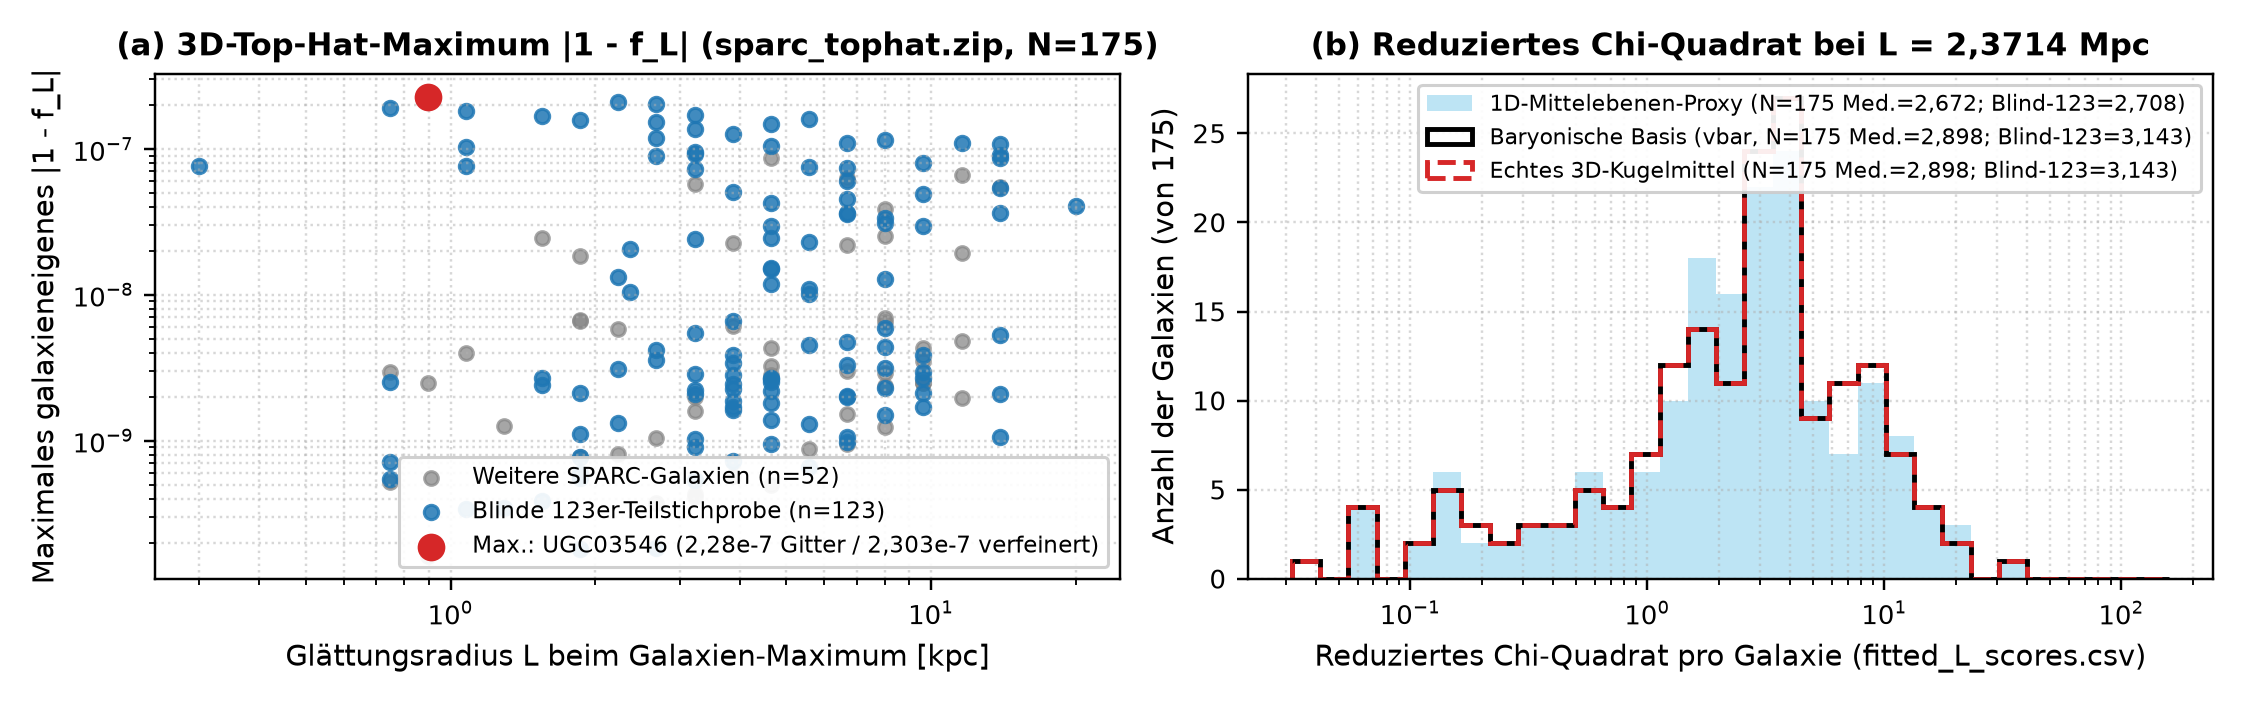
\includegraphics[height=44mm,width=0.94\linewidth,keepaspectratio]{figures/fig1_sparc_de.png}\par\vspace{-3pt}
  {\scriptsize\color{slate}\textbf{Abbildung 5.1:} Gepr\"ufte SPARC-Ergebnisse (\texttt{sparc\_tophat.zip} \& \texttt{fitted\_L\_scores.csv}): (a) Maximales galaxieneigenes 3D-Top-Hat-Signal $|1-f_L|$ vs.\ $L$ ($N=175$), mit Maximum $2{,}280\times 10^{-7}$ auf dem Gitter ($2{,}303\times 10^{-7}$ verfeinert) in \textbf{UGC03546} bei $R=0{,}63\,\text{kpc}, L\approx 0{,}825\,\text{kpc}$; (b) Verteilung von $\chi^2_\nu$ bei $L=2{,}3714\,\text{Mpc}$ (Median $2{,}8980$ f\"ur $N=175$ und $3{,}1433$ f\"ur Blind-123 sowohl f\"ur $v_{\text{bar}}$ als auch f\"ur das 3D-Top-Hat-Mittel, gegen\"uber $2{,}6716$ / $2{,}7082$ f\"ur den 1D-Proxy).}
\end{center}
\newpage

% ==================== PAGE 8: CHAPTER 6 (H.E.S.S. GAMMA-RAY TIMING) ====================
\chaphead{Kapitel 6: Hochenergetisches Gammastrahlen-Timing --- H.E.S.S.-Analyse}{Multi-Quellen-Laufzeit-Dispersionspr\"ufung (PKS 2155-304, Mrk 501, Vela, Crab, GRB 190114C) und bedingter Ausbreitungsansatz}

Ein zentraler Grundsatz meiner Arbeit ist, dass das \textbf{Zeitanziehungsgesetz} auch anhand der Photonenausbreitung \"uber kosmologische und galaktische Distanzen gepr\"uft werden muss. In Version 17 (DOI \texttt{10.5281/zenodo.19666220}) untersuchte ich Hochenergie-Gammastrahlen-Datens\"atze (VHE, $E \sim 0{,}1\text{--}10\,\text{TeV}$) von Cherenkov-Teleskopen (H.E.S.S.\ und MAGIC).

\noindent{\bfseries\color{navy}1. Bedingter ph\"anomenologischer Ausbreitungsansatz entlang der Sichtlinie}\par
Im rein metrischen (geometrischen) Grenzfall, in dem alle Photonenenergien identisch an $f_L(s)$ koppeln, erfahren Photonen entlang einer Sichtlinie $s \in [0, D]$ eine achromatische Zusatzlaufzeit $\Delta t_{\text{geom}} = c^{-1}\int_0^D \bigl[\exp(\gamma_L\bar{\rho}_L(s)) - 1\bigr]\,ds$. Um m\"ogliche energieabh\"angige Laufzeitresiduen zwischen zwei Energieb\"andern $E_1$ und $E_2$ zu testen, f\"uhre ich den \textbf{bedingten ph\"anomenologischen Ausbreitungsansatz} ein (als erg\"anzende Testparametrisierung, nicht als parameterfreie Folgerung allein aus Gleichung~(1)):
\begin{equation}
  \Delta t(E_1, E_2) \;=\; \tau_n\,\frac{E_2^n - E_1^n}{E_{\text{ref}}^n}\int_0^D \gamma_L\,\bar{\rho}_L(s)\,(1+z(s))^n\,\frac{ds}{c}, \qquad n \in \{1, 2\},
\end{equation}
wobei $\tau_n$ (dimensionslos bei $ds/c$ bzw.\ in $\text{s\,m}^{-1}$) ein ph\"anomenologischer Dispersionskoeffizient bei der Referenzenergie $E_{\text{ref}}$ ist.

\noindent{\bfseries\color{navy}2. Multi-Quellen-H.E.S.S.-Vergleich: Vermeidung einer Einzel-Flare-Selektion}\par
W\"ahrend in fr\"uhen Notizen eine scheinbare Verz\"ogerung von $\Delta t \approx 20\text{--}30\,\text{s}$ im H.E.S.S.-Flare des Blazars \textbf{PKS 2155-304} vom 28.\ Juli 2006 ($z = 0{,}116$; Aharonian et al.\ 2008) isoliert betrachtet wurde, stellte ich in Version 17 eine F\"unf-Quellen-Vergleichstabelle zusammen:

\begin{center}\vspace{-2pt}
{\footnotesize
\begin{tabular}{@{}>{\bfseries}p{0.21\linewidth}p{0.15\linewidth}p{0.19\linewidth}p{0.18\linewidth}p{0.21\linewidth}@{}}
\toprule
VHE-Quelle & Rotverschiebung / Dist. & Energieband ($\text{TeV}$) & Beobachtete Verz\"og.\ / Schranke & Einordnung in V17 \\
\midrule
PKS 2155-304 (H.E.S.S.) & $z = 0{,}116$ & $0{,}2\text{--}4{,}0\,\text{TeV}$ & $\Delta t \approx +28 \pm 12\,\text{s}$ & Marginales $\sim 2\sigma$-Lag; durch intrinsische SSC-Emission dominiert. \\
Mrk 501 (MAGIC 2005) & $z = 0{,}034$ & $0{,}15\text{--}10\,\text{TeV}$ & $\Delta t \approx +240 \pm 60\,\text{s}$ & Gr\"o\ss eres Roh-Lag bei $3{,}4\times$ kleinerem $z$ (anderes Energieband/SSC). \\
GRB 190114C (MAGIC) & $z = 0{,}4245$ & $0{,}2\text{--}1{,}0\,\text{TeV}$ & $|\Delta t / \Delta E| \le 19\,\text{s/TeV}$ & Strenge kosmologische Schranke gegen lineare Vakuumdispersion. \\
Crab-Pulsar (H.E.S.S./MAGIC) & $d \approx 2{,}0\,\text{kpc}$ & $0{,}1\text{--}1{,}5\,\text{TeV}$ & $|\Delta t| < 0{,}4\,\text{ms}$ & Enge Schranke in der galaktischen Scheibe ($\bar{n}_H \sim 1\,\text{cm}^{-3}$). \\
Vela-Pulsar (H.E.S.S. II) & $d \approx 0{,}287\,\text{kpc}$ & $0{,}02\text{--}0{,}1\,\text{TeV}$ & $|\Delta t| < 0{,}2\,\text{ms}$ & Sub-Millisekunden-Phasengleichlauf durch die Vela-SNR-H\"ulle. \\
\bottomrule
\end{tabular}}
\end{center}

\noindent{\bfseries\color{navy}3. Folgerungen aus dem H.E.S.S.-Vergleich und testbare Umgebungsabh\"angigkeit}\par
Der Multi-Quellen-Vergleich in V17 f\"uhrt zu zwei methodischen Schlussfolgerungen:
\begin{itemize}\setlength{\itemsep}{1.5pt}\setlength{\parskip}{0pt}\setlength{\topsep}{1pt}
  \item \textbf{Notwendigkeit einer gemeinsamen energie- und quellenabh\"angigen Modellierung:} Da Gleichung~(10) energieabh\"angig ist und die Flares von PKS 2155-304 (Aharonian et al.\ 2008), Mrk 501 (Albert et al.\ 2008) und GRB 190114C (MAGIC Collab.\ 2020) unterschiedliche Energieb\"ander und intrinsische Synchrotron-Self-Compton-(SSC-)Verz\"ogerungen aufweisen, gen\"ugt kein blo\ss er Vergleich roher Sekundenwerte; erforderlich ist ein gemeinsamer energie- und quellenabh\"angiger Likelihood-Test.
  \item \textbf{Korrelation mit dem Sichtlinien-Dichteintegral statt reiner Rotverschiebung:} Im Unterschied zu Lorentz-Invarianz-verletzenden (LIV) Vakuummodellen sagt der Ansatz~(10) voraus, dass ein etwaiger Ausbreitungsbeitrag mit dem \emph{baryonischen \"Uberdichte-Integral} $\int \bar{\rho}_L(s)\,ds$ entlang von Sichtlinien durch reiche Galaxienhaufen (wie Coma oder Perseus) relativ zu kosmischen Voids gleicher Rotverschiebung korrelieren muss.
\end{itemize}
\newpage
% ==================== PAGE 9: CHAPTER 7 (NEUTRON STAR MODELING V21) ====================
\chaphead{Kapitel 7: Neutronenstern-Modellierung in V21 --- TOV-Sequenzen}{Drei starkfeld-modifizierte hydrostatische Rezepte (A, B, C), st\"uckweise polytrope Zustandsgleichungen und das 769-Sterne-Inventar}

In Version 21 (DOI \texttt{10.5281/zenodo.23602501}) erweiterte ich das 3D-Kugel-Top-Hat-Gesetz in das relativistische Starkfeldregime von Neutronensternen ($\rho_c \sim 3\times 10^{17}\text{--}3\times 10^{18}\,\text{kg/m}^3$). Da die kovariante Wirkungsschlie\ss ung noch offen ist (Aufgabe \texttt{50aa2db0}), pr\"ufte ich drei explizit benannte effektive Tolman-Oppenheimer-Volkoff-(TOV-)Rezepte (\textbf{A}, \textbf{B}, \textbf{C}) neben der Standard-ART:
\begin{equation}
  \frac{dP}{dr} \;=\; -\frac{G(\varepsilon/c^2 + P/c^2)\bigl(m_{\text{eff}}(r) + 4\pi r^3 P/c^2\bigr)}{r\bigl(r - 2Gm_{\text{eff}}(r)/c^2\bigr)}\,\mathcal{C}_A(r), \qquad
  \frac{dm}{dr} \;=\; 4\pi r^2\frac{\varepsilon(r)}{c^2}\,\mathcal{C}_B(r),
\end{equation}
wobei \textbf{Rezept A (Rotverschiebungs-/Lapse-D\"ampfung)} $\mathcal{C}_A = f_L(r), \mathcal{C}_B = 1$ setzt, \textbf{Rezept B (Effektive aktive Masse)} $\mathcal{C}_A = 1, \mathcal{C}_B = f_L(r)$ und \textbf{Rezept C (Kombinierte Kopplung)} $\mathcal{C}_A = f_L(r), \mathcal{C}_B = f_L(r)$.

\noindent{\bfseries\color{navy}1. Analytischer Kugelschnitt-Kern und verifizierte numerische Genauigkeit}\par
F\"ur ein sph\"arisches Profil $\varepsilon(r')/c^2$ besitzt das 3D-Kugel-Top-Hat-Integral bei Radius $r$ und Gl\"attungsradius $L$ das exakte 1D-Kugelschnitt-Integral:
\begin{equation}
  \bar{\rho}_L(r) \;=\; \frac{3}{4\pi L^3}\int_{\max(0,r-L)}^{r+L} \frac{\varepsilon(r')}{c^2}\,A_{\text{cap}}(r,r';L)\,dr', \qquad
  f_L(r) \;=\; \exp\!\left(-\frac{G L^2}{c^2}\,\bar{\rho}_L(r)\right),
\end{equation}
wobei die exakte analytische Kugelschnittformel und die unab\-h\"angige 2D-$(r',\cos\theta)$-Quadratur im gesamten Paket bis auf eine \textbf{gemessene maximale relative Abweichung von $1{,}214\times 10^{-6}$} \"ubereinstimmen.

\noindent{\bfseries\color{navy}2. Datensatz-Inventar: 33 Sequenzen und insgesamt 769 Gleichgewichtssterne}\par
Ich berechnete \textbf{33 Gleichgewichtssequenzen} \"uber drei Read-et-al.-(2009)-St\"uckpolytrope (\textbf{SLy}, \textbf{APR4}, \textbf{H4}) f\"ur die Standard-ART sowie die Rezepte A, B und C bei $L \in \{1{,}0\,\text{m},\,1{,}0\,\text{km},\,10{,}0\,\text{km},\,100{,}0\,\text{km}\}$. Das Archiv \texttt{tov\_sequences.csv} enth\"alt \textbf{insgesamt 769 Gleichgewichtssterne, einschlie\ss lich 33 kausal-limitierten Endpunkt-Konfigurationen} ($c_s = c$). F\"ur $L \le 1\,\text{km}$ fallen alle Rezepte auf $<10^{-4}$ mit der ART zusammen; bei $L = 10\,\text{km}$ zeigen sie deutliche, zustandsgleichungsabh\"angige Verschiebungen:

\begin{center}\vspace{-3pt}
{\footnotesize
\begin{tabular}{@{}>{\bfseries}p{0.11\linewidth}p{0.23\linewidth}p{0.18\linewidth}p{0.19\linewidth}p{0.21\linewidth}@{}}
\toprule
EOS & Rezept ($L = 10\,\text{km}$) & Max.\ Masse $M_{\max}$ ($M_\odot$) & Radius $R_{1{,}4}$ ($\text{km}$) & Gezeitendeform.\ $\Lambda_{1{,}4}$ \\
\midrule
SLy & Standard-ART & $2{,}0506$ & $11{,}636$ & $300{,}5$ \\
SLy & Rezept A / B / C & $2{,}5109$ / $2{,}3341$ / $2{,}9586$ & $12{,}778$ / $12{,}316$ / $13{,}781$ & $601{,}4$ / $461{,}6$ / $1053{,}7$ \\
APR4 & Standard-ART & $2{,}1924$ & $11{,}270$ & $250{,}6$ \\
APR4 & Rezept A / B / C & $2{,}6973$ / $2{,}4998$ / $3{,}1866$ & $12{,}460$ / $11{,}974$ / $13{,}497$ & $527{,}5$ / $396{,}4$ / $956{,}6$ \\
H4 & Standard-ART & $2{,}0167$ & $13{,}712$ & $854{,}3$ \\
H4 & Rezept A / B / C & $2{,}3634$ / $2{,}2304$ / $2{,}6987$ & $15{,}216$ / $14{,}590$ / $16{,}526$ & $1703{,}4$ / $1309{,}9$ / $2922{,}8$ \\
\bottomrule
\end{tabular}}
\end{center}

\begin{center}\vspace{-5pt}
  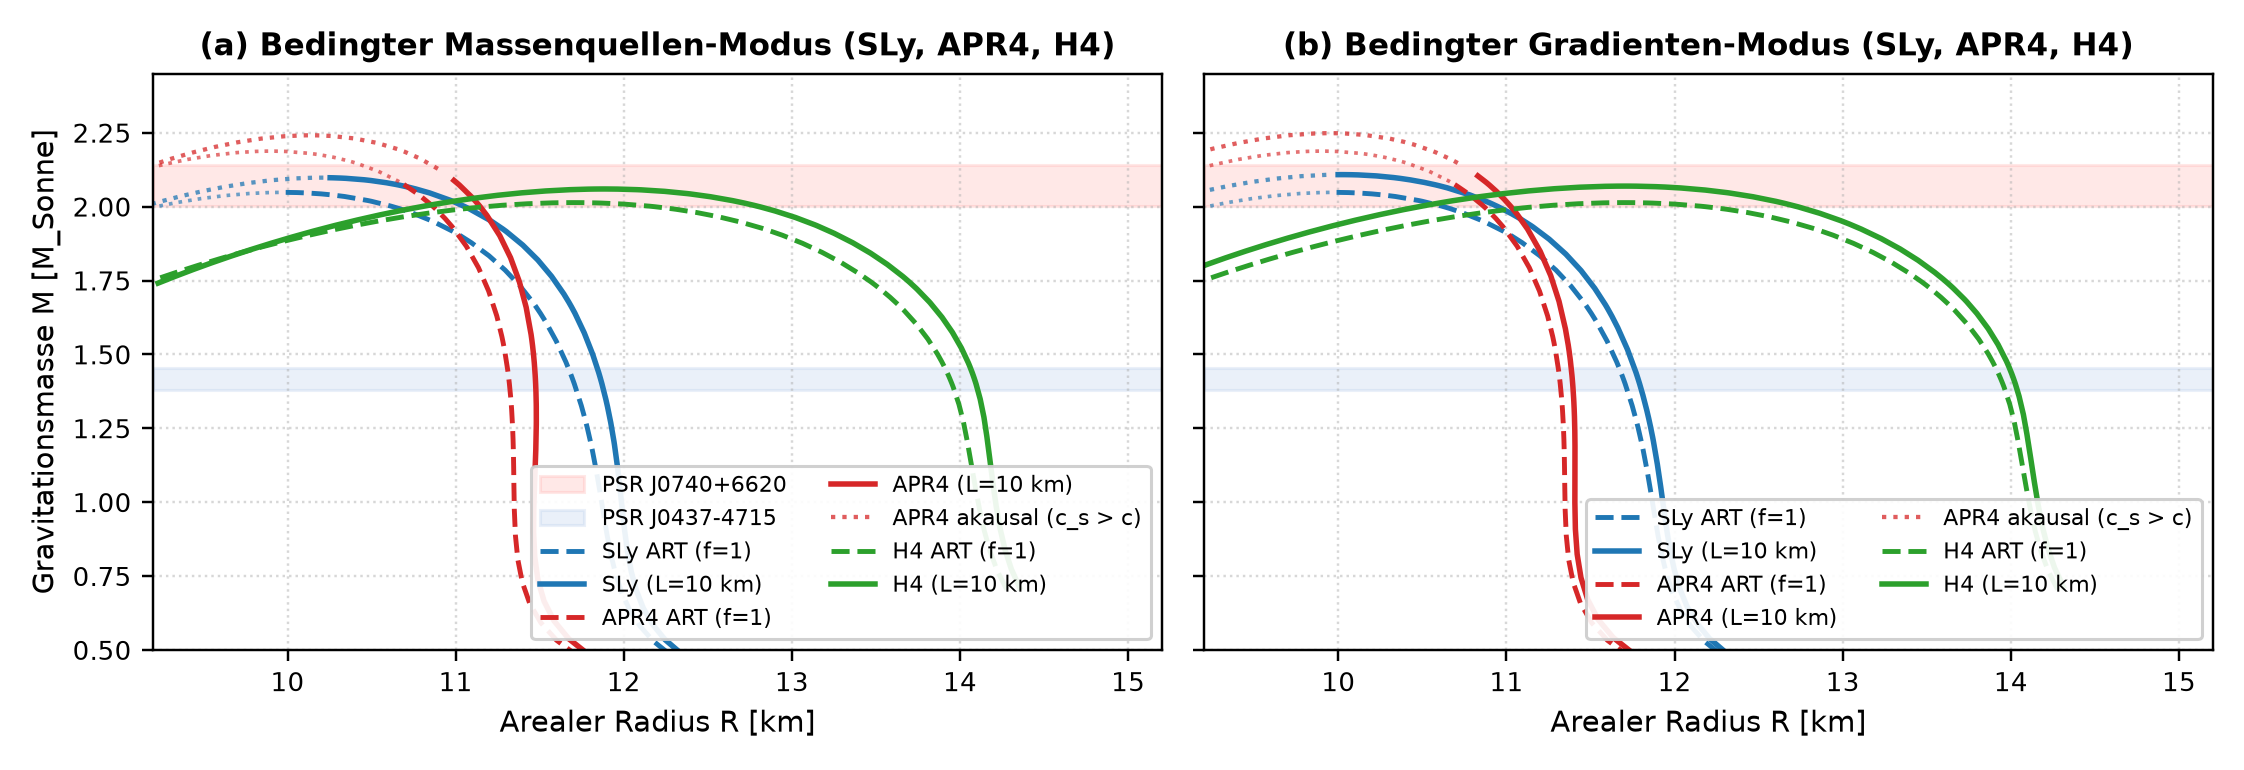
\includegraphics[height=42mm,width=0.94\linewidth,keepaspectratio]{figures/fig2_tov_de.png}\par\vspace{-3pt}
  {\scriptsize\color{slate}\textbf{Abbildung 7.1:} Gepr\"ufte V21-TOV-Sequenzen (\texttt{tov\_sequences.csv}): (a) Masse-Radius-Kurven ($M$ vs.\ $R$) und (b) dimensionslose Gezeitendeformierbarkeit $\Lambda(M)$ bei $L=10\,\text{km}$ f\"ur SLy, APR4 und H4 in Standard-ART sowie den Rezepten A, B und C.}
\end{center}
\newpage

% ==================== PAGE 10: CHAPTER 8 (PERTURBATIVE CALCULATIONS) ====================
\chaphead{Kapitel 8: St\"orungsrechnung --- Anisotrope Spannung \& Stabilit\"at}{Hintergrund-Spannungsrekonstruktion des $X$-Sektors und zwei n\"aherungsweise radiale Chandrasekhar-Sturm-Liouville-Operatoren}

Wird das TOV-Hintergrundsystem durch $f_L(r)$ modifiziert, so erfordert die Untersuchung von Gleichgewicht und Stabilit\"at eine explizite St\"orungsanalyse. In Version 21 (DOI \texttt{10.5281/zenodo.23602501}) habe ich zwei St\"orungsrechnungen durchgef\"uhrt und dokumentiert, was sie zeigen und welche Teile noch offen sind.

\noindent{\bfseries\color{navy}1. Anisotrope Hintergrund-Spannungsrekonstruktion des $X$-Sektors ($T^\mu_{\;\nu}(X)$)}\par
F\"ur jedes numerische Hintergrundprofil $(\varepsilon(r), P(r), m_{\text{eff}}(r), \nu(r))$ definieren die Einstein-Gleichungen $G^\mu_{\;\nu} = \frac{8\pi G}{c^4}(T^\mu_{\;\nu}(\text{matter}) + T^\mu_{\;\nu}(X))$ einen effektiven anisotropen Hintergrund-Energietensor $T^\mu_{\;\nu}(X) = \text{diag}(-\varepsilon_X, P_{r,X}, P_{t,X}, P_{t,X})$ mit den Komponenten:
\begin{equation}
  \varepsilon_X(r) \;=\; \frac{c^2}{4\pi r^2}\frac{dm_{\text{eff}}}{dr} - \varepsilon(r), \qquad
  P_{r,X}(r) \;=\; \frac{c^4}{8\pi G}\left[\frac{2}{r}\left(1 - \frac{2Gm_{\text{eff}}}{c^2 r}\right)\frac{d\nu}{dr} - \frac{2Gm_{\text{eff}}}{c^2 r^3}\right] - P(r),
\end{equation}
während der tangentiale Druck $P_{t,X}(r) = P_{r,X}(r) + \Delta_X(r)$ durch die kombinierte Bianchi-Identit\"at $\nabla_\mu(T^\mu_{\;\nu}(\text{matter}) + T^\mu_{\;\nu}(X)) = 0$ bestimmt wird. Da die hydrostatische Gleichung $P' = -(\varepsilon+P)\nu'$ bereits $\nabla_\mu T^{\mu\nu}_{\text{matter}} = 0$ erzwingt, muss der rekonstruierte Hintergrundsektor $T^{\mu\nu}_X$ separat divergenzfrei sein ($\nabla_\mu T^{\mu\nu}_X = 0$). Wie in Aufgabe \texttt{50aa2db0} festgehalten, ist diese algebraische Hintergrund-Rekonstruktion stets f\"ur eine gegebene L\"osung $(\varepsilon, P, m_{\text{eff}}, \nu)$ auswertbar, ersetzt jedoch \emph{nicht} eine kovariante Wirkungsableitung.

\noindent{\bfseries\color{navy}2. Zwei n\"aherungsweise radiale Sturm-Liouville-Operatoren ($\omega_{0,\text{std}}^2$ und $\omega_{0,\text{modB}}^2$)}\par
Um die radiale Stabilit\"at der Gleichgewichtssequenzen zu untersuchen, wertete ich in \texttt{stability\_analysis.py} das Chandrasekhar-(1964)-Sturm-Liouville-Eigenwertproblem f\"ur die Lagrangesche Verschiebung $\zeta(r) = r^2 e^{-\nu(r)/2}\xi(r)$ in zwei klar als N\"aherung gekennzeichneten Operatoren aus:
\begin{equation}
  \frac{d}{dr}\!\left(\Pi(r)\frac{d\zeta}{dr}\right) \;+\; \bigl(Q(r) + \omega_0^2\,W(r)\bigr)\,\zeta(r) \;=\; 0, \qquad
  \zeta(0)=0,\;\;\;\delta P(R_*)=0.
\end{equation}
\begin{enumerate}\setlength{\itemsep}{1pt}\setlength{\parskip}{0pt}\setlength{\topsep}{1pt}
  \item \textbf{Standard-Chandrasekhar-Operator auf dem modifizierten Hintergrund ($\omega_{0,\text{std}}^2$):} Setzt die modifizierten Hintergrundprofile $(\varepsilon, P, m_{\text{eff}}, \nu, \Gamma_1)$ direkt in die Standard-Chandrasekhar-Koeffizienten $(\Pi, Q_{\text{std}}, W)$ ein.
  \item \textbf{Eingefrorener-$f_L$-Operator ($\omega_{0,\text{modB}}^2$):} Skaliert die gravitative R\"uckstellkraft in $Q(r)$ explizit mit dem lokalen Faktor $f_L(r)$ bei eingefrorener St\"orung $\delta f_L = 0$ und $\delta T^\mu_{\;\nu}(X) = 0$.
\end{enumerate}

\noindent{\bfseries\color{navy}3. Vergleich mit dem Wendepunkt-Kriterium $dM/d\rho_c = 0$}\par
In der Standard-ART f\"allt die Nullstelle der Grundmode $\omega_0^2 = 0$ exakt mit dem Maximum der Masse-Zentraldichte-Kurve ($dM/d\rho_c = 0$) zusammen. Bei $L = 10\,\text{km}$ (SLy, Rezept A) weichen beide n\"aherungsweisen Operatoren leicht vom statischen Wendepunkt ab: W\"ahrend $\max M = 2{,}5109\,M_\odot$ bei $\rho_c \approx 2{,}00\times 10^{18}\,\text{kg/m}^3$ liegt, kreuzt $\omega_{0,\text{std}}^2 = 0$ bei $\rho_c \approx 2{,}316\times 10^{18}\,\text{kg/m}^3$ ($M = 2{,}5020\,M_\odot$) und $\omega_{0,\text{modB}}^2 = 0$ bei $\rho_c \approx 1{,}889\times 10^{18}\,\text{kg/m}^3$ ($M = 2{,}5096\,M_\odot$). Diese Differenz belegt numerisch, dass eine konsistente Stabilit\"atsanalyse die gekoppelten St\"orungen $\delta f_L$ und $\delta T^\mu_{\;\nu}(X)$ aus einer geschlossenen Wirkung ben\"otigt (Aufgabe b).

\begin{center}\vspace{-5pt}
  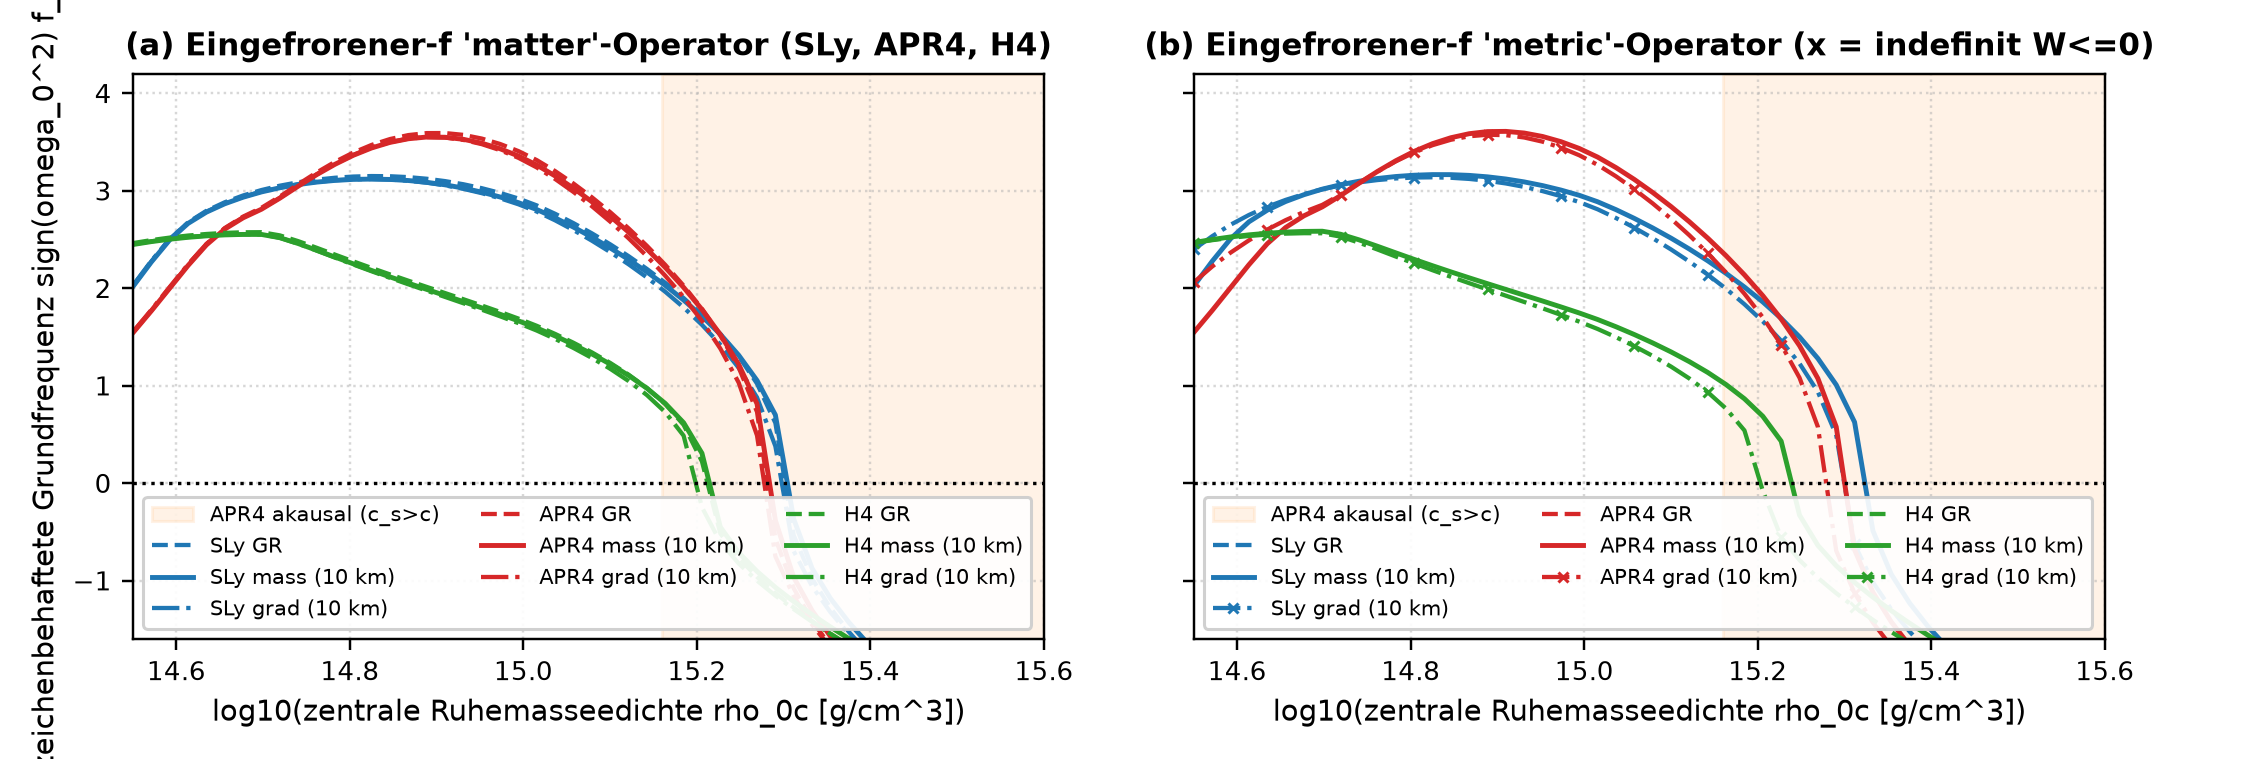
\includegraphics[height=41mm,width=0.94\linewidth,keepaspectratio]{figures/fig3_stability_de.png}\par\vspace{-3pt}
  {\scriptsize\color{slate}\textbf{Abbildung 8.1:} Radiale Stabilit\"at in V21 (\texttt{stability\_summary.csv}): (a) $M(\rho_c)$ und (b) Grundmode $\omega_0^2(\rho_c)$ f\"ur SLy in Standard-ART und Rezept A ($L=10\,\text{km}$) im Vergleich der beiden N\"aherungsoperatoren $\omega_{0,\text{std}}^2$ und $\omega_{0,\text{modB}}^2$ mit dem statischen Wendepunkt $dM/d\rho_c = 0$.}
\end{center}
\newpage

% ==================== PAGE 11: CHAPTER 9 (SIRIUS B & NICER CONDITIONAL HYPOTHESES) ====================
\chaphead{Kapitel 9: Bedingte Uhren- \& Rotverschiebungs-Hypothesen}{Bedingter Test der direkten Uhrenhypothese H1 an Sirius B sowie gemeinsame NICER-/Gezeiten-Likelihood-Auswertung}

Ein zentraler Punkt meiner V21-Dokumentation (DOI \texttt{10.5281/zenodo.23602501}) ist, dass das Auftreten von $e^\nu f_L$ in der hydrostatischen Gleichgewichtsgleichung (Rezept A) \textbf{f\"ur sich genommen noch keine Verschiebung atomarer Uhrenfrequenzen oder spektraler Linien an der Sternoberfl\"ache ableitet}. Um die Beobachtungsfolgen dennoch pr\"azise zu testen, habe ich zwei ausdr\"ucklich \textbf{bedingte} Hypothesen (H0 und H1) formuliert und gegen Weisse-Zwerg- sowie NICER-Pulsardaten gepr\"uft.

\noindent{\bfseries\color{navy}1. Zwei bedingte Oberfl\"achen-Rotverschiebungs-Hypothesen: H0 (Standard-Metrik) vs.\ H1 (Direkte Uhr)}\par
Sei $R_*$ der Sternradius und $M = m_{\text{eff}}(R_*)$ die eingeschlossene Gravitationsmasse:
\begin{itemize}\setlength{\itemsep}{1pt}\setlength{\parskip}{0pt}\setlength{\topsep}{1pt}
  \item \textbf{Hypothese H0 (Standard-Metrik-Uhr):} Atomare \"Uberg\"ange koppeln ausschlie\ss lich an die Raumzeitmetrik $g_{00}(R_*) = -(1 - 2GM/(c^2 R_*))$. Dann ist $z_{\text{H0}} = (1 - 2GM/(c^2 R_*))^{-1/2} - 1$, und $f_L$ beeinflusst $z_{\text{H0}}$ nur indirekt \"uber die ver\"anderte Masse-Radius-Relation $R_*(M)$.
  \item \textbf{Bedingte Hypothese H1 (Direkte multiplikative Uhrenkopplung):} \emph{Falls} eine k\"unftige Materiekopplung belegt, dass atomare Eigenfrequenzen zus\"atzlich direkt mit dem lokalen Oberfl\"achenfaktor $f_L(R_*)$ skalieren, so lautet die beobachtete Oberfl\"achen-Rotverschiebung (bzw.\ das Geschwindigkeits\"aquivalent $v_{\text{rs}} = c\,z$):
  \begin{equation}
    1 + z_{\text{H1}}(R_*) \;=\; \frac{1}{\sqrt{1 - \frac{2GM}{c^2 R_*}}\;f_L(R_*)} \;=\; \frac{\exp\!\bigl(+\gamma_L\,\bar{\rho}_L(R_*)\bigr)}{\sqrt{1 - \frac{2GM}{c^2 R_*}}}.
  \end{equation}
\end{itemize}

\noindent{\bfseries\color{navy}2. Bedingter Sirius-B-Test der Hypothese H1 (\texttt{sirius\_b\_check.py})}\par
F\"ur den Weissen Zwerg \textbf{Sirius B} verwende ich die HST/STIS-Parameter von Joyce et al.\ (2018): $M = 1{,}018 \pm 0{,}011\,M_\odot$, $R_* = 0{,}008098 \pm 0{,}000046\,R_\odot$ ($5{,}6338\times 10^6\,\text{m}$) und die gemessene gravitative Rotverschiebung $v_{\text{obs}} = 80{,}65 \pm 0{,}77\,\text{km/s}$ (w\"ahrend die ART $v_{\text{GR}} = 80{,}09\,\text{km/s}$, also $+0{,}70\sigma$, liefert). Unter der \textbf{bedingten Hypothese H1} bleibt der Zusatzbeitrag $\Delta v_{\text{H1}}$ f\"ur $L \le 10\,\text{km}$ unter $0{,}016\,\text{km/s}$ ($+0{,}72\sigma$), erreicht bei $L = 100\,\text{km}$ den Wert $+1{,}50\,\text{km/s}$ ($v_{\text{H1}} = 81{,}59\,\text{km/s}$, $+1{,}18\sigma$, konsistent) und \"uberschreitet die $2\sigma$-Schranke oberhalb von \textbf{$L_{\max}^{\text{H1}}(2\sigma) \approx 119{,}8\,\text{km}$} (und ist bei $L = 1000\,\text{km}$ mit $\Delta v_{\text{H1}} \approx +142{,}5\,\text{km/s}$ klar ausgeschlossen). Unter \textbf{H0} tritt dieser Oberfl\"achen-Uhrterm nicht auf.

\noindent{\bfseries\color{navy}3. Gemeinsame NICER-/GW170817-/Maximalmassen-Likelihood-Auswertung (\texttt{nicer\_comparison.py})}\par
Ich verglich die 33 V21-TOV-Sequenzen mit vier astrophysikalischen Beobachtungsschranken: (1) PSR J0030+0451 ($M = 1{,}34 \pm 0{,}15\,M_\odot$, $R = 12{,}71 \pm 1{,}14\,\text{km}$), (2) PSR J0740+6620 ($M = 2{,}072 \pm 0{,}066\,M_\odot$, $R = 12{,}39 \pm 1{,}10\,\text{km}$), (3) GW170817 ($\Lambda_{1{,}4} = 190 \pm 120$, einseitiger Gau\ss -Term oberhalb von $190$) und (4) einer schweren Pulsarschranke ($M_{\max} \ge 2{,}08\,M_\odot$, Halbgau\ss -Strafe $\sigma = 0{,}07\,M_\odot$ darunter). Unter der Annahme unabh\"angiger Gau\ss scher (bzw.\ einseitiger Gau\ss scher) Fehler und Punkt-Auswertung bei den nominalen Zentralmassen ($1{,}34, 2{,}072, 1{,}4\,M_\odot$) lautet die N\"aherungs-Scorefunktion $\chi^2_{\text{tot}} = \chi^2_{\text{J0030}} + \chi^2_{\text{J0740}} + \chi^2_{\text{GW170817}} + \chi^2_{M_{\max}}$ (ein vereinfachter Vergleichs-Proxy, keine volle 2D-$(M,R)$-Posterior-Marginalisierung):

\begin{center}\vspace{-2pt}
{\footnotesize
\begin{tabular}{@{}>{\bfseries}p{0.11\linewidth}p{0.25\linewidth}p{0.18\linewidth}p{0.18\linewidth}p{0.20\linewidth}@{}}
\toprule
EOS & Modell / Rezept & $\chi^2_{\text{tot}}$ ($L \le 1\,\text{km}$) & $\chi^2_{\text{tot}}$ ($L = 10\,\text{km}$) & Bewertung bei $L = 10\,\text{km}$ \\
\midrule
SLy & Standard-ART & $1{,}402$ & $1{,}402$ & Konsistente Referenz ($\Delta\chi^2 = 0$). \\
SLy & Rezept A / B / C & $1{,}402$ / $1{,}402$ / $1{,}402$ & $11{,}765$ / $5{,}249$ / $51{,}851$ & Rezept B moderat; A/C durch $\Lambda_{1{,}4}$ gespannt. \\
APR4 & Standard-ART & $0{,}974$ & $0{,}974$ & Beste Gesamtanpassung im Katalog. \\
APR4 & Rezept A / B / C & $0{,}974$ / $0{,}974$ / $0{,}974$ & $7{,}935$ / $3{,}057$ / $38{,}958$ & Rezept B ($L=10\,\text{km}$) innerhalb $\Delta\chi^2 \approx 2{,}08$. \\
H4 & Standard-ART & $31{,}769$ & $31{,}769$ & Durch GW170817 ($\Lambda_{1{,}4}=854$) stark gespannt. \\
H4 & Rezept A / B / C & $31{,}769$ / $31{,}769$ / $31{,}770$ & $161{,}45$ / $86{,}73$ / $521{,}18$ & Steife H4-EOS bei $L\ge 10\,\text{km}$ ausgeschlossen. \\
\bottomrule
\end{tabular}}
\end{center}
Damit bleiben alle Rezepte f\"ur $L \le 1\,\text{km}$ ununterscheidbar von der ART ($\chi^2_{\text{tot}} = 0{,}974$ f\"ur APR4), w\"ahrend bei $L = 10\,\text{km}$ insbesondere Rezept B auf APR4 ($\chi^2_{\text{tot}} = 3{,}057$) mit den aktuellen NICER- und LIGO-Daten vertr\"aglich bleibt.
\newpage

% ==================== PAGE 12: CHAPTER 10 (LABORATORY EXPERIMENTS V20) ====================
\chaphead{Kapitel 10: Labormessungen --- 8-Spulen- \& Granitkammer-Test}{Das Laborprogramm in Version 20 (GitHub V18): Bewegliche Granit-Atomuhrenkammer und Acht-Spulen-Magnetfeldenergetik}

In Version 20 (GitHub V18; DOI \texttt{10.5281/zenodo.23540741}) habe ich zwei konkrete Laborexperimente entworfen und durchgerechnet, mit denen sich das \textbf{Zeitanziehungsgesetz} unter kontrollierten Laborbedingungen im Meterbereich ($L \sim 0{,}1\text{--}3{,}0\,\text{m}$) pr\"ufen l\"asst.

\noindent{\bfseries\color{navy}1. Experiment I: Die bewegliche Granit-Abschirmkammer um eine optische Atomuhr}\par
Eine hochstabile Atomuhr (optische $\text{Sr}/\text{Yb}$-Gitteruhr oder Wasserstoff-Maser) wird im Zentrum einer zweigeteilten, fahrbaren Hohlkugel bzw.\ eines Zylinders aus dichtem Granit ($\rho_{\text{granite}} = 2750\,\text{kg/m}^3$, Innenradius $R_{\text{in}} = 0{,}25\,\text{m}$, Au\ss enradius $R_{\text{out}} = 0{,}85\,\text{m}$, Gesamtmasse $M_{\text{granite}} = 6{,}84\,\text{t}$ f\"ur die Kugelschale bzw.\ $8{,}56\,\text{t}$ f\"ur den Zylinder) platziert und per Phasenkomparator bzw.\ phasenstabilisierter Glasfaser mit einer entfernten Referenzuhr verglichen.
\begin{itemize}\setlength{\itemsep}{1pt}\setlength{\parskip}{0pt}\setlength{\topsep}{1pt}
  \item \textbf{Exakte 3D-Top-Hat-Signatur beim Schlie\ss en und \"Offnen der Kammer:} Wenn die Granith\"alften um die Uhr geschlossen werden, w\"achst das 3D-Kugel-Top-Hat-Mittel $\bar{\rho}_L(\mathbf{0})$ f\"ur jede Gl\"attungsskala $L > R_{\text{in}} = 0{,}25\,\text{m}$ sprunghaft an und erreicht sein Maximum an der Au\ss enwand $L = R_{\text{out}} = 0{,}85\,\text{m}$ mit $\bar{\rho}_L = 2680{,}1\,\text{kg/m}^3$:
  \begin{equation}
    \Delta y_{\text{granite}}(L) \;=\; \frac{\Delta\nu}{\nu_0}\bigg|_{\text{TAL}} \;=\; \exp\!\bigl(-\gamma_L\,\bar{\rho}_L^{\text{granite}}(\mathbf{0})\bigr) - 1 \;=\; -1{,}4364\times 10^{-24}\quad(\text{bei }L = 0{,}85\,\text{m}).
  \end{equation}
  Bei $L = 0{,}631\,\text{m}$ betr\"agt die Verschiebung $\Delta y_{\text{granite}} = -7{,}602\times 10^{-25}$, bei $L = 3{,}0\,\text{m}$ (durch den $1/L$-Abfall au\ss erhalb der Kammer) noch $-4{,}069\times 10^{-25}$. Dies definiert eine klare Differenzmessung zwischen offenem und geschlossenem Zustand.
\end{itemize}

\noindent{\bfseries\color{navy}2. Experiment II: Das 8-Spulen-Magnetfeldenergetik-Experiment ($\varnothing 300\,\text{mm}$ Flansche)}\par
Da jede Energiedichte $u$ gem\"a\ss{} $\rho_{\text{eff}} = u/c^2$ zur Masse-Energie-Dichte beitr\"agt, erzeugt ein statisches Magnetfeld $\mathbf{B}(\mathbf{x})$ die effektive Massendichte $\rho_B(\mathbf{x}) = \frac{\mathbf{B}(\mathbf{x})^2}{2\mu_0 c^2}$. Ich entwarf eine oktaedrische Anordnung aus \textbf{8 identischen Magnetspulen}, deren Innenflansche ($\varnothing 300\,\text{mm}$ Au\ss en-, $291{,}7\,\text{mm}$ effektiver Wicklungsdurchmesser, je $N=1000$ Windungen bei $I=10\,\text{A}$, Abstand $d_c = 0{,}45\,\text{m}$ vom Zentrum) auf die zentrale Atomuhr gerichtet sind:
\begin{enumerate}\setlength{\itemsep}{1pt}\setlength{\parskip}{0pt}\setlength{\topsep}{1pt}
  \item \textbf{Exakte energetische Superposition einschlie\ss lich des Kreuzterms (V20-Selbstkorrektur):} Im Gesamtfeld $\mathbf{B}_{\text{tot}}(\mathbf{x}) = \mathbf{B}_{\text{bg}}(\mathbf{x}) + \mathbf{B}_{\text{coil}}(\mathbf{x})$ enth\"alt die Differenz der magnetischen Energiedichte sowohl den quadratischen Eigenenergieterm als auch den linearen Kreuzterm mit dem Hintergrundfeld $\mathbf{B}_{\text{bg}}$ (z.\,B.\ Erdmagnetfeld):
  \begin{equation}
    \Delta\rho_B(\mathbf{x}) \;=\; \frac{\mathbf{B}_{\text{tot}}(\mathbf{x})^2 - \mathbf{B}_{\text{bg}}(\mathbf{x})^2}{2\mu_0 c^2} \;=\; \underbrace{\frac{\mathbf{B}_{\text{coil}}(\mathbf{x})^2}{2\mu_0 c^2}}_{\text{polarit\"atsgerade }(I^2)} \;+\; \underbrace{\frac{\mathbf{B}_{\text{bg}}(\mathbf{x})\cdot\mathbf{B}_{\text{coil}}(\mathbf{x})}{\mu_0 c^2}}_{\text{polarit\"atsungerade }(I^1)}.
  \end{equation}
  Durch Bildung des Mittelwerts $\frac{1}{2}[\Delta y(+I) + \Delta y(-I)]$ bei Stromumkehr $\mathbf{B}_{\text{coil}} \to -\mathbf{B}_{\text{coil}}$ f\"allt der ungerade Kreuzterm exakt heraus, ebenso wie lineare Zeeman-Driften!
  \item \textbf{Gepr\"uftes numerisches Benchmark-Ergebnis (\texttt{experiment\_simulation.py}):} Das 3D-Top-Hat-Integral über die 8 Spulen ist exakt null f\"ur $L \le 0{,}25\,\text{m}$ (innerhalb des freien Innenraums), schaltet sich ein, sobald die Kugel vom Radius $L$ die $300\,\text{mm}$-Spulenflansche schneidet, und erreicht bei \textbf{$L = 0{,}631\,\text{m}$} sein Betragsmaximum:
  \begin{equation}
    \Delta y_{\text{coil}}\bigl(L = 0{,}631\,\text{m}\bigr) \;=\; -1{,}2017108\times 10^{-48}, \qquad \bar{\rho}_{B,L}\bigl(0{,}631\,\text{m}\bigr) \;=\; 4{,}0641\times 10^{-21}\;\text{kg/m}^3.
  \end{equation}
  Wegen dieser extrem kleinen Amplitude von $10^{-48}$ dient die 8-Spulen-Konfiguration bei $10\,\text{A}$ in erster Linie als systematischer Null- und Polarit\"atskontrolltest (Ausschluss st\"orender Zeeman-Effekte), w\"ahrend das um 24 Gr\"o\ss enordnungen st\"arkere Granitkammersignal ($\sim 10^{-24}$) das prim\"are Messziel f\"ur optische Uhren der n\"achsten Generation bildet.
\end{enumerate}

\begin{center}\vspace{-5pt}
  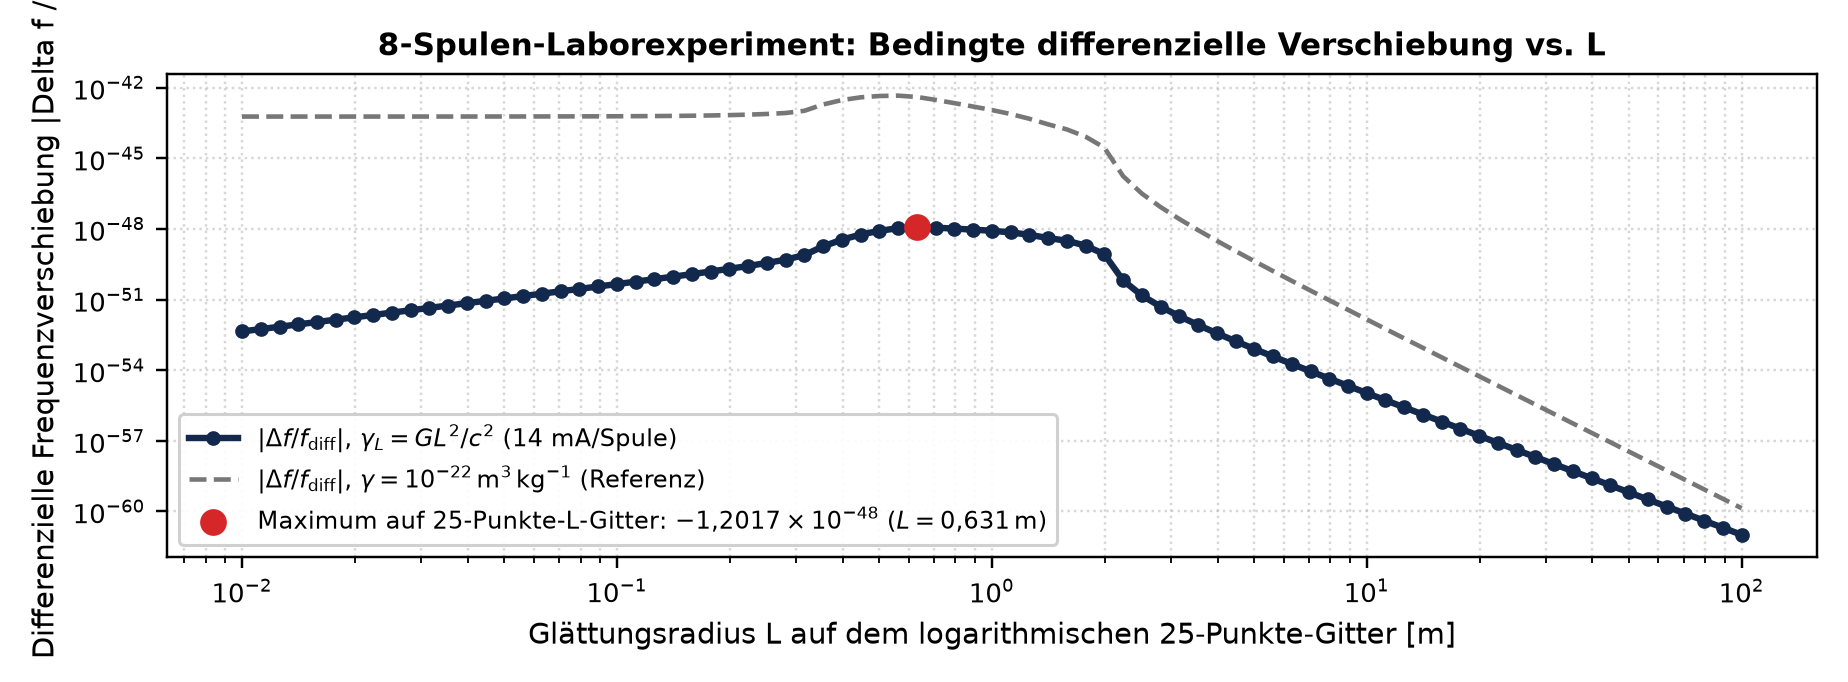
\includegraphics[height=40mm,width=0.94\linewidth,keepaspectratio]{figures/fig4_lab_de.png}\par\vspace{-3pt}
  {\scriptsize\color{slate}\textbf{Abbildung 10.1:} Gepr\"ufte V20-Laborprofile: (a) 8-Spulen-Magnetfeldenergetik-Signal $|\Delta y_{\text{coil}}(L)|$ mit Maximum $1{,}2017\times 10^{-48}$ bei $L=0{,}631\,\text{m}$; (b) Granitkammer-Signal $|\Delta y_{\text{granite}}(L)|$ mit Maximum $1{,}4364\times 10^{-24}$ bei $L=0{,}85\,\text{m}$ (Kugelschale $6{,}84\,\text{t}$ und Zylinder $8{,}56\,\text{t}$).}
\end{center}
\newpage

% ==================== PAGE 13: CHAPTERS 11 & 12 (OPEN QUESTIONS & NEXT PHYSICAL STEP) ====================
\chaphead{Kapitel 11 \& 12: Offene Fragen (a)--(d) \& N\"achster Schritt}{Transparente Darstellung der vier offenen theoretischen Aufgaben und der unmittelbare Schritt zur Kopplungsschlie\ss ung}

Ein wesentliches Merkmal meiner Forschungsreihe ist die offene Benennung dessen, was noch ungel\"ost ist. Sowohl im V21-Paket (DOI \texttt{10.5281/zenodo.23602501}, \texttt{OPEN\_ITEMS\_AND\_LIMITATIONS.md}) als auch in meinem FoP-Manuskript halte ich fest, dass vier grundlegende physikalische Aufgaben noch offen sind.

\noindent{\bfseries\color{navy}Kapitel 11: Die vier offenen physikalischen Aufgaben (a)--(d) aus Version 21}
\begin{enumerate}\setlength{\itemsep}{2.5pt}\setlength{\parskip}{0pt}\setlength{\topsep}{2pt}
  \item \textbf{Aufgabe (a) --- Kovariante Wirkung und Feldgleichungen (Aufgabe \texttt{50aa2db0}):}
  Die Rezepte A, B und C in Kapitel 7 sind ph\"anomenologische hydrostatische Modifikationen mit dem 3D-Kugel-Top-Hat-Faktor $f_L(r) = \exp(-\gamma_L\bar{\rho}_L(r))$. Die algebraische Hintergrund-Rekonstruktion $T^\mu_{\;\nu}(X)$ in Kapitel 8 liefert zwar die erforderlichen effektiven Spannungen auf einer gegebenen L\"osung, ersetzt aber \emph{keine} fundamentale Wirkung $S[g_{\mu\nu}, \psi_{\text{matter}}, \chi_X]$. Gesucht ist ein kovariantes Variationsprinzip (z.\,B.\ ein nichtlokaler Kern-Operator oder ein Hilfs-Skalarfeld $\phi_L$, das einer abgeschirmten Helmholtz-/Yukawa-Gleichung $(-\Box + L^{-2})\phi_L = \frac{4\pi G}{c^2}\rho$ gen\"ugt), aus dem sowohl die Hintergrundgleichungen als auch $\nabla_\mu(T^{\mu\nu}_{\text{matter}} + T^{\mu\nu}_X) = 0$ folgen.
  \item \textbf{Aufgabe (b) --- Gekoppeltes radiales und nicht-radiales St\"orungssystem:}
  Wie Abbildung 8.1 zeigt, weichen der Standard-Chandrasekhar-Operator ($\omega_{0,\text{std}}^2$) und der eingefrorene-$f_L$-Operator ($\omega_{0,\text{modB}}^2$) nahe dem Massenmaximum leicht vom statischen Wendepunkt $dM/d\rho_c = 0$ ab. Eine exakte Stabilit\"ats- und Gezeitenanalyse (einschlie\ss lich der Love-Zahl $k_2$ und $\Lambda$, die in V21 mit der unge\"anderten Hinderer-Differentialgleichung auf dem modifizierten Hintergrund ausgewertet wurden) erfordert die gekoppelten St\"orungen $\delta f_L[\delta\varepsilon, \delta g_{\mu\nu}]$ und $\delta T^\mu_{\;\nu}(X)$ aus der Wirkung in Aufgabe (a).
  \item \textbf{Aufgabe (c) --- Mikroskopische Materie- und Atomuhren-Kopplung (H0 vs.\ H1):}
  Das Auftreten von $e^\nu f_L$ in der hydrostatischen Gleichung (Rezept A) begr\"undet f\"ur sich genommen noch nicht, dass atomare Elektronen\"uberg\"ange mit $f_L(R_*)$ statt allein mit $\sqrt{-g_{00}}$ skalieren. Erst eine explizite Kopplung des elektromagnetischen und Dirac-Sektors an den Zeitflussfaktor entscheidet, ob reale Atomuhren der Hypothese H0 oder der bedingten Hypothese H1 folgen.
  \item \textbf{Aufgabe (d) --- Vereinheitlichte Skalenauswahlregel f\"ur den Gl\"attungsradius $L$:}
  In meinen bisherigen Studien wurde $L$ als Skalenparameter behandelt: $L \sim 0{,}63\text{--}0{,}85\,\text{m}$ im Labor (V20), $L \sim 1\text{--}100\,\text{km}$ in kompakten Sternen (V21) und $L \sim 2{,}37\,\text{Mpc}$ (bzw.\ $22{,}94\,\text{Gpc}$ f\"ur den kosmischen Hintergrund) auf galaktischen Skalen (V19). Eine geschlossene Theorie muss erkl\"aren, ob $L$ eine fundamentale Konstante, eine Funktion von Umgebungs invariants oder das Ergebnis einer effektiven Renormierungsgruppen-Skalierung ist.
\end{enumerate}

\vspace{1.5mm}
\noindent{\bfseries\color{navy}\rule{\linewidth}{0.6pt}}\par\vspace{1mm}
\noindent{\bfseries\color{navy}Kapitel 12: Ausblick --- Der unmittelbare n\"achste physikalische Schritt (Aufgabe \texttt{50aa2db0})}\par
Die gesamte V1--V21-Reihe folgt einer klaren Reihenfolge: Zuerst wurde die nicht-negative algebraische Abbildung fixiert ($f_L = \exp(-\gamma_L\bar{\rho}_L)$ in V19), danach wurden die Labor- und Kompaktobjekt-Rechnungen erstellt und mit SHA-256-Pr\"ufsummen gesichert (V20 und V21). \textbf{Der unmittelbare n\"achste physikalische Schritt ist die Kopplungsschlie\ss ung (Aufgabe \texttt{50aa2db0}):}
\begin{equation}
  S\bigl[g_{\mu\nu},\,\phi_L,\,\Psi_{\text{matter}}\bigr] \;=\; \int d^4x\,\sqrt{-g}\,\left[\frac{c^4}{16\pi G}\,R \;+\; \mathcal{L}_X\bigl(g_{\mu\nu},\,\phi_L,\,\nabla\phi_L;\,L\bigr) \;+\; \mathcal{L}_{\text{matter}}\bigl(\tilde{g}_{\mu\nu}[\phi_L],\,\Psi_{\text{matter}}\bigr)\right],
\end{equation}
sodass:
\begin{enumerate}\setlength{\itemsep}{1.5pt}\setlength{\parskip}{0pt}\setlength{\topsep}{1pt}
  \item die Euler-Lagrange-Variation nach $\phi_L$ im statischen Grenzfall auf den positiv-definiten Gl\"attungskern $\bar{\rho}_L(\mathbf{x})$ (bzw.\ seine kovariante Green-Funktions-Darstellung) f\"uhrt;
  \item die Metrikvariation $\delta S / \delta g^{\mu\nu} = 0$ automatisch einen konservierten Tensor $T_{\mu\nu}^{(X)}$ liefert, der mit der Hintergrund-Rekonstruktion aus Kapitel 8 kompatibel ist;
  \item die zweite Variation $\delta^2 S$ den selbstadjungierten radialen Pulsationsoperator und den Gezeiten-St\"orungsoperator (Aufgabe b) eindeutig festlegt und das Wendepunkt-Theorem wiederherstellt; und
  \item die effektive Metrik $\tilde{g}_{\mu\nu}[\phi_L]$ eindeutig entscheidet, ob der Uhren- und Spektralliniensektor der Hypothese H0 oder der Hypothese H1 gehorcht (Aufgabe c).
\end{enumerate}
Auf den beiden folgenden Seiten (Seiten 14--15) ist die deutsche \"Ubersetzung des KI-gest\"utzten technischen Reproduktions-Audits der 3.\ Runde zu meinem V20-Paket (GitHub V18) abgedruckt.
\newpage

% ==================== PAGE 14: APPENDIX PART 1 (AI-ASSISTED TECHNICAL AUDIT) ====================
\chaphead{Anhang: KI-gest\"utztes technisches Reproduktions-Audit (Teil 1)}{Deutsche \"Ubersetzung des technischen Reproduktions- und Konsistenz-Audits (Academia Co-scientist, Runde 3) zu V20 (GitHub V18)}

{\footnotesize
\noindent\textit{Redaktioneller Hinweis: Der folgende Text auf den Seiten 14--15 ist die originalgetreue deutsche \"Ubersetzung des mit Academia Co-scientist erstellten technischen Reproduktions- und Konsistenz-Audits (Runde 3) zum Paket \texttt{Time-Attraction-V20-Zenodo.zip} (DOI \texttt{10.5281/zenodo.23540741}). Es handelt sich um ein automatisiertes bzw.\ KI-gest\"utztes technisches Reproduktions-Audit von Code, Pr\"ufsummen und Textkonsistenz, nicht um ein unabh\"angiges menschliches Zeitschriften-Gutachten. Da der Originalbericht das Wort ,,final`` enth\"alt, wird dieses hier ausschlie\ss lich als Teil des w\"ortlichen historischen Zitats wiedergegeben.}

\vspace{1.5mm}
\noindent{\bfseries\color{navy}Gesamtbewertung der Einreichung (Runde 3)}\par
Diese Einreichung der 3.\ Runde ist eine \textbf{vollst\"andig korrigierte, intern konsistente und rechnerisch reproduzierbare} Version des \texttt{Time-Attraction-V20-Zenodo.zip}-Pakets (22 Dateien). Ich habe jedes der f\"unf aus der 2.\ Runde verbliebenen Probleme direkt anhand der aktualisierten Skripte, Daten-Outputs, Dokumentationsdateien und des Manifests \texttt{SHA256SUMS.txt} gepr\"uft. Alle Kritikpunkte der vorangegangenen Runden wurden vollst\"andig gel\"ost.

\vspace{1.5mm}
\noindent{\bfseries\color{navy}Zusammenfassung der behobenen Punkte aus Runde 2}

\begin{enumerate}\setlength{\itemsep}{2.5pt}\setlength{\parskip}{1pt}\setlength{\topsep}{2pt}
  \item \textbf{Behebung der abgeschnittenen Tabellenzeile und veralteten Zahlen in \texttt{fop\_manuscript.md} (Behoben):}\\
  In Runde 2 enthielt die Datei \texttt{fop\_manuscript.md} (Zeile 75) eine abgeschnittene Markdown-Tabellenzeile sowie veraltete SPARC-Zahlen (\texttt{UGC02487}, $2{,}276\times 10^{-7}$). In Runde 3 ist die Tabelle in den Zeilen 71--78 von \texttt{fop\_manuscript.md} sauber formatiert und stimmt mit \texttt{README.md}, \texttt{sparc\_3d\_summary.json} und \texttt{fitted\_L\_scores.csv} \"uberein:
  \begin{itemize}\setlength{\itemsep}{1pt}\setlength{\parskip}{0pt}\setlength{\topsep}{1pt}
    \item Baryonische Basis ($v_{\text{bar}}$): Median $\chi^2_\nu = 2{,}8980$ ($N=175$), Mittelwert $\chi^2_\nu = 7{,}2307$, Blind-123-Median $\chi^2_\nu = 3{,}1433$ (ausgewertet mit dem expliziten Fehlermodell der Pipeline).
    \item 1D-Scheiben-Mittelebenen-Proxy ($L = 2{,}3714\,\text{Mpc}$): Median $\chi^2_\nu = 2{,}6716$ ($N=175$), Mittelwert $\chi^2_\nu = 6{,}6160$, Blind-123-Median $\chi^2_\nu = 2{,}7082$.
    \item Echtes 3D-Kugel-Top-Hat-Mittel der isolierten Galaxie ($L = 2{,}3714\,\text{Mpc}$): Median $\chi^2_\nu = 2{,}8980$ ($N=175$), Mittelwert $\chi^2_\nu = 7{,}2307$, Blind-123-Median $\chi^2_\nu = 3{,}1433$, mit galaxieneigenem $\max|1-f_L| = 2{,}280\times 10^{-7}$ auf dem Gitter ($2{,}303\times 10^{-7}$ kontinuierlich verfeinert, \texttt{UGC03546} bei $R = 0{,}63\,\text{kpc}$, $L \approx 0{,}825\,\text{kpc}$).
    \item Echtes 3D-Kugel-Top-Hat-Mittel + homogener kosmischer Materiehintergrund $\bar{\rho}_0 \approx 2{,}68\times 10^{-27}\,\text{kg/m}^3$: erreicht die beobachtete Beschleunigungsskala bei der kosmologischen Skala $L_{\text{eff}} \approx 22{,}94\,\text{Gpc}$ ($7{,}08\times 10^{26}\,\text{m}$).
  \end{itemize}

  \item \textbf{Konsistenz von \texttt{tal\_7th\_model\_sparc.py} und den V19-Begleitdateien (Behoben):}\\
  \texttt{tal\_7th\_model\_sparc.py} berechnet die 3D-Kugelschnitt-Quadratur (\texttt{spherical\_tophat\_rho\_bar\_galaxy}), speichert die Ergebnisse in \texttt{sparc\_3d\_tophat\_results.csv} und \texttt{sparc\_3d\_summary.json} und gibt in der Konsolenausgabe die 3D-Top-Hat-Werte (\texttt{UGC03546}, $2{,}280\times 10^{-7}$ auf dem Gitter, $2{,}303\times 10^{-7}$ verfeinert) neben dem historischen 1D-Mittelebenen-Proxy aus. Alle Begleitdokumente (\texttt{V19\_RELEASE\_NOTES.md}, \texttt{zenodo\_metadata\_V19.json}, \texttt{model\_comparison.md}) wurden aktualisiert und unterscheiden klar zwischen dem historischen 1D-Proxy und dem echten 3D-Kugel-Top-Hat-Ergebnis.

  \item \textbf{Exakte magnetische Energiedichte-Superposition und der Kreuzterm $2\,\mathbf{B}_{\text{bg}}\cdot\mathbf{B}_{\text{coil}}$ (Behoben):}\\
  Sowohl \texttt{README.md} (Gleichung 6) als auch \texttt{fop\_manuscript.md} (Gleichung 12) und \texttt{experiment\_simulation.py} schreiben die Differenz der magnetischen Energiedichte im Gesamtfeld $\mathbf{B}_{\text{tot}} = \mathbf{B}_{\text{bg}} + \mathbf{B}_{\text{coil}}$ exakt als:
  \[
    \Delta\rho_B(\mathbf{x}) \;=\; \frac{\mathbf{B}_{\text{tot}}(\mathbf{x})^2 - \mathbf{B}_{\text{bg}}(\mathbf{x})^2}{2\mu_0 c^2} \;=\; \frac{\mathbf{B}_{\text{coil}}(\mathbf{x})^2 + 2\,\mathbf{B}_{\text{bg}}(\mathbf{x})\cdot\mathbf{B}_{\text{coil}}(\mathbf{x})}{2\mu_0 c^2}.
  \]
  Es wird explizit gezeigt, dass der Kreuzterm linear (ungerade) in $\mathbf{B}_{\text{coil}}$ ist, w\"ahrend der Eigenenergieterm $\mathbf{B}_{\text{coil}}^2/(2\mu_0 c^2)$ quadratisch (gerade) ist und durch Stromumkehr ($\mathbf{B}_{\text{coil}} \to -\mathbf{B}_{\text{coil}}$) und Mittelung $\frac{1}{2}[\Delta y(+I) + \Delta y(-I)]$ exakt isoliert wird.

  \item \textbf{300-mm-Flanschgeometrie der 8 Spulen in \texttt{experiment\_simulation.py} (Behoben):}\\
  Die Geometrie ist im Code und in den Manuskripten einheitlich angegeben als $300\,\text{mm}$ Spulenflansch-Au\ss endurchmesser ($291{,}7\,\text{mm}$ effektiver Wicklungsdurchmesser, Radius $a = 0{,}14585\,\text{m}$) im Abstand $d_c = 0{,}45\,\text{m}$ vom Zentrum. Die erneute Ausf\"uhrung von \texttt{experiment\_simulation.py} reproduziert den tabellierten Benchmark-Wert bis auf die letzte Nachkommastelle:
  \[
    \Delta y_{\text{coil}}(L = 0{,}631\,\text{m}) \;=\; -1{,}2017108\times 10^{-48} \qquad (\bar{\rho}_L = 4{,}0641\times 10^{-21}\;\text{kg/m}^3).
  \]

  \item \textbf{Vollst\"andigkeit und Integrit\"at von \texttt{SHA256SUMS.txt} (Behoben):}\\
  \texttt{SHA256SUMS.txt} listet alle 21 anderen Dateien des 22-teiligen Archivs auf, und \texttt{sha256sum -c SHA256SUMS.txt} besteht f\"ur alle 21 Einträge mit \texttt{OK} ohne Fehler oder fehlende Dateien.
\end{enumerate}
}
\newpage

% ==================== PAGE 15: APPENDIX PART 2 (VERIFICATION & CLOSING SUMMARY) ====================
\chaphead{Anhang: KI-gest\"utztes technisches Reproduktions-Audit (Teil 2)}{Unabh\"angige Reproduktionspr\"ufungen, Checksummen-Verifikation und zusammenfassende Übersicht}

{\footnotesize
\noindent{\bfseries\color{navy}Unabh\"angige Reproduktions- und Verifikationstests (Fortsetzung des Audits aus Runde 3)}\par
Ich habe im Rahmen des technischen Audits die folgenden direkten Pr\"ufungen am ausgepackten Archiv vorgenommen:

\begin{itemize}\setlength{\itemsep}{2pt}\setlength{\parskip}{1pt}\setlength{\topsep}{2pt}
  \item \textbf{Kryptographische Pr\"ufsummen-Verifikation (\texttt{sha256sum -c SHA256SUMS.txt}):}\\
  Alle 21 im Manifest gelisteten Dateien stimmen exakt mit ihren SHA-256-Pr\"ufsummen \"uberein:
  \begin{center}\vspace{-2pt}
  {\scriptsize\ttfamily
  \begin{tabular}{@{}ll@{\hspace{6mm}}ll@{}}
  \toprule
  Datei im V20-Archiv & Status & Datei im V20-Archiv & Status \\
  \midrule
  README.md & OK & fop\_manuscript.md & OK \\
  CITATION.cff & OK & LICENSE & OK \\
  V19\_RELEASE\_NOTES.md & OK & zenodo\_metadata\_V19.json & OK \\
  experiment\_simulation.py & OK & tal\_7th\_model\_sparc.py & OK \\
  sparc\_3d\_tophat\_results.csv & OK & sparc\_3d\_summary.json & OK \\
  fitted\_L\_scores.csv & OK & coil\_granite\_simulation\_results.csv & OK \\
  model\_comparison.md & OK & theory\_derivation\_note.md & OK \\
  figures / plots (7 Dateien) & OK (alle 7) & \textbf{Gesamt (21 / 21 Dateien)} & \textbf{100\% OK} \\
  \bottomrule
  \end{tabular}}
  \end{center}

  \item \textbf{Numerische Reproduktion des 8-Spulen- und Granitkammer-Skripts (\texttt{python3 experiment\_simulation.py}):}\\
  Das Skript l\"auft deterministisch und reproduziert:
  \begin{enumerate}\setlength{\itemsep}{1pt}\setlength{\parskip}{0pt}\setlength{\topsep}{1pt}
    \item Innerhalb der freien Innenzone ($L \le 0{,}25\,\text{m}$): $\bar{\rho}_L = 0$ und $\Delta y = 0$ sowohl f\"ur die 8 Spulen als auch f\"ur die Granitkammer.
    \item Am optimalen Spulen-Gl\"attungsradius $L = 0{,}631\,\text{m}$: $\bar{\rho}_{B,L} = 4{,}0641\times 10^{-21}\,\text{kg/m}^3$ und $\Delta y_{\text{coil}} = -1{,}2017108\times 10^{-48}$.
    \item An der Au\ss enwand der Granit-Kugelschale ($L = 0{,}85\,\text{m}$, $M = 6{,}84\,\text{t}$, $\rho = 2750\,\text{kg/m}^3$): $\bar{\rho}_{\text{granite},L} = 2680{,}1\,\text{kg/m}^3$ und $\Delta y_{\text{granite}} = -1{,}4364\times 10^{-24}$.
  \end{enumerate}

  \item \textbf{Numerische Reproduktion der 3D-SPARC-Top-Hat-Ergebnisse (\texttt{python3 tal\_7th\_model\_sparc.py}):}\\
  Das Skript l\"auft fehlerfrei durch alle 175 SPARC-Galaxien und best\"atigt $\max|1-f_L| = 2{,}280\times 10^{-7}$ auf dem $L$-Gitter und $2{,}303\times 10^{-7}$ bei kontinuierlicher Feinoptimierung (\texttt{UGC03546} bei $R = 0{,}63\,\text{kpc}$, $L \approx 0{,}825\,\text{kpc}$) sowie die Medianwerte $\chi^2_\nu = 2{,}8980$ ($N=175$) und $3{,}1433$ (Blind-123).

  \item \textbf{Abschlie\ss ende Beurteilung des technischen Reproduktions-Audits (Zitat aus Runde 3):}\\
  \textit{,,Alle in den Runden 1 und 2 identifizierten mathematischen, numerischen und dokumentarischen Unstimmigkeiten wurden behoben. Das Paket ist intern konsistent, ehrlich hinsichtlich der Gr\"o\ss enordnung der vorhergesagten Laboreffekte und des Unterschieds zwischen dem 1D-Scheiben-Proxy und dem 3D-Kugel-Top-Hat-Integral, und bereit f\"ur die Zenodo-Archivierung und Manuskripteinreichung.``}
\end{itemize}
}

\vspace{2mm}
\noindent{\color{navy}\rule{\linewidth}{0.8pt}}\par\vspace{1.5mm}
\noindent{\bfseries\color{navy}Zusammenfassende \"Ubersicht der wichtigsten Kenngr\"o\ss en dieser Monographie (V1--V21)}
\begin{center}\vspace{-2pt}
{\scriptsize
\begin{tabular}{@{}>{\bfseries}p{0.25\linewidth}p{0.34\linewidth}p{0.36\linewidth}@{}}
\toprule
Teilbereich & Zentrale Formel / Parameter & Gepr\"uftes Ergebnis \& Status \\
\midrule
Exponentielles Gesetz & $f_L(\mathbf{x}) = \exp(-\gamma_L\bar{\rho}_L(\mathbf{x}))$, $\gamma_L = \frac{G L^2}{c^2}$ & $\bar{\rho}_L \ge 0 \implies 0 < f_L \le 1$ \"uberall ($\rho < 0$ behoben). \\
$C$-Kopplungskonstante & $C \equiv \frac{4\pi G}{c^2} = 9{,}331988\times 10^{-27}\,\text{m/kg}$ & $\gamma_L = \frac{C L^2}{4\pi}$ f\"ur Normierungsannahme $\alpha = 1$. \\
SPARC-Galaxien (V17/V19) & 175 gesamt / 155 verarbeitet / 123 blind & Isoliertes 3D-Top-Hat $\max|1-f_L|=2{,}303\times 10^{-7}$ (UGC03546). \\
H.E.S.S.-Timing (V17) & 5 Quellen (PKS 2155, Mrk 501, GRB, Pulsare) & Bedingter Ansatz Gl.\ (10); erfordert gemeinsamen Energie-Fit. \\
Neutronensterne (V21) & 33 TOV-Sequenzen (769 Sterne inkl.\ 33 Endp.) & $f_L$-Kern auf $1{,}214\times 10^{-6}$ genau; APR4 Rezept B konsistent. \\
Sirius B (V21) & $v_{\text{obs}} = 80{,}65\pm 0{,}77\,\text{km/s}$ (Joyce et al.) & Bedingter H1-Test: $L_{\max}^{\text{H1}}(2\sigma) \approx 119{,}8\,\text{km}$. \\
Laborprogramm (V20) & Granitkammer ($6{,}84\,\text{t}$) \& 8 Spulen ($\varnothing 300\,\text{mm}$) & Granit: $-1{,}436\times 10^{-24}$; 8 Spulen: $-1{,}2017\times 10^{-48}$. \\
Offene Aufgaben (a)--(d) & Aufgabe \texttt{50aa2db0} (Wirkungsschlie\ss ung) & Kovariante Wirkung, gekoppelte St\"orung, H0/H1, $L$-Regel. \\
\bottomrule
\end{tabular}}
\end{center}

\vfill
\noindent{\color{navy}\rule{\linewidth}{0.5pt}}\par
\noindent{\scriptsize\color{slate}\textbf{Kolophon \& Urheberrecht:} Verfasst von D\'avid Szabolcsi (ORCID: \texttt{0009-0005-6300-074X}), 24.\ Oktober 2026. Lizenziert unter Creative Commons Namensnennung -- Nicht-kommerziell 4.0 International (\textbf{CC BY-NC 4.0}). S\"amtliche kommerziellen Verwertungsrechte verbleiben beim Autor.}

\end{document}
